\documentclass[xetex,mathserif,serif,aspectratio=169]{beamer}

\usepackage{xltxtra}
\usepackage{color}
\usepackage{url}
\usepackage{listings}
\usepackage{fontspec}
\usepackage{geometry}
\usepackage{lastpage}
\usepackage{fancyhdr}
\usepackage{amsmath}
\usepackage{amsthm}
\usepackage{amssymb}
\usepackage{blkarray}
\usepackage{multicol}
\usepackage{relsize}
\usepackage{listings}
\usepackage{xunicode}
\usepackage{xltxtra}
\usepackage{color}
\usepackage{url}
\usefonttheme[onlymath]{serif}

\definecolor{solarized@base03}{HTML}{002B36}
\definecolor{solarized@base02}{HTML}{073642}
\definecolor{solarized@base01}{HTML}{586e75}
\definecolor{solarized@base00}{HTML}{657b83}
\definecolor{solarized@base0}{HTML}{839496}
\definecolor{solarized@base1}{HTML}{93a1a1}
\definecolor{solarized@base2}{HTML}{EEE8D5}
\definecolor{solarized@base3}{HTML}{FDF6E3}
\definecolor{solarized@yellow}{HTML}{B58900}
\definecolor{solarized@orange}{HTML}{CB4B16}
\definecolor{solarized@red}{HTML}{DC322F}
\definecolor{solarized@magenta}{HTML}{D33682}
\definecolor{solarized@violet}{HTML}{6C71C4}
\definecolor{solarized@blue}{HTML}{268BD2}
\definecolor{solarized@cyan}{HTML}{2AA198}
\definecolor{solarized@green}{HTML}{859900}
\definecolor{yaleblue}{HTML}{0E4C92}

\newcommand{\yellow}[1]{\textcolor{solarized@yellow}{#1}}
\newcommand{\orange}[1]{\textcolor{solarized@orange}{#1}}
\newcommand{\red}[1]{\textcolor{solarized@red}{#1}}
\newcommand{\magenta}[1]{\textcolor{solarized@magenta}{#1}}
\newcommand{\violet}[1]{\textcolor{solarized@violet}{#1}}
\newcommand{\blue}[1]{\textcolor{solarized@blue}{#1}}
\newcommand{\cyan}[1]{\textcolor{solarized@cyan}{#1}}
\newcommand{\green}[1]{\textcolor{solarized@green}{#1}}
\newcommand{\yblue}[1]{\textcolor{yaleblue}{#1}}
\newcommand{\base}[1]{\textcolor{solarized@base01}{#1}}


\defaultfontfeatures{Mapping=tex-text}
\hypersetup{pdfstartview={FitH}}

\newcommand{\old}[1]{\fontspec[Alternate=1,Ligatures={Common}]{Hoefler Text}\fontsize{18pt}{30pt}\selectfont #1}%
\newcommand{\oldA}[1]{\fontspec[Alternate=1,Ligatures={Common, Rare}]{Hoefler Text}\fontsize{12pt}{15pt}\selectfont #1}%
\newcommand{\oldB}[1]{\fontspec[Ligatures={Common}]{Didot}\fontsize{12pt}{15pt}\color{solarized@base02}\selectfont #1}%
\newcommand{\tfont}[1]{\fontspec[Alternate=1,Ligatures={Common}]{Hoefler Text}\fontsize{12pt}{20pt}\selectfont #1}%
\newcommand{\dfont}[1]{\fontspec[Ligatures={Common}]{Didot}\fontsize{12pt}{12pt}\selectfont #1}%

\setbeamerfont{title}{family=\old}
\setbeamerfont{author}{family=\tfont}%
\setbeamerfont{frametitle}{family=\oldA}
\setbeamerfont{date}{family=\dfont}

\setbeamertemplate{navigation symbols}{}
\setbeamertemplate{footline}[text line]{%
  \parbox{0.99\linewidth}{
    \normalsize\vspace*{-24pt}\hfill{\color{solarized@base00}\insertframenumber/\inserttotalframenumber}
  }
}


\setlength{\parindent}{0pt}
\setlength{\parskip}{12pt}

\setbeamercolor{structure}{bg=solarized@base3, fg=solarized@base02}
\setbeamercolor{titlelike}{fg=solarized@cyan}
\setbeamercolor{title}{fg=solarized@blue}
\setbeamercolor{subtitle}{fg=solarized@magenta}
\setbeamercolor{alerted text}{fg=orange}
\setbeamercolor{itemize}{fg=solarized@base02}
\setbeamercolor{background canvas}{bg=solarized@base3}
\setbeamercolor{enumerate subitem}{fg=solarized@base02}

\newcommand{\minimize}{\mathop{\mathrm{minimize}}}
\newcommand{\argmin}{\mathop{\mathrm{arg\,min}}}
\newcommand{\argmax}{\mathop{\mathrm{arg\,max}}}
\newcommand{\st}{\mathop{\mathrm{subject\,\,to}}}


\usepackage[]{algorithm2e}
\usepackage{../kbordermatrix}

\begin{document}

%%%%%%%%%%%%%%%%%%%%%%%%%%%%%%%%%%%%%%%%%%%%%%%%%%%
\begin{frame}[fragile] \frametitle{} \oldB \small

\vfill

{\fontsize{0.7cm}{0cm}\selectfont Lecture 16 \\\vspace{0.2cm}
Neural Network Software}\\\vspace{0.5cm}
28 March 2016

\vspace{2cm}

\begin{minipage}{0.6\textwidth}
Taylor B. Arnold \\
Yale Statistics \\
STAT 365/665
\end{minipage}
\hfill
\begin{minipage}{0.3\textwidth}\raggedleft

\includegraphics[scale=0.3]{../yale-logo.png}
\end{minipage}%

\end{frame}

%%%%%%%%%%%%%%%%%%%%%%%%%%%%%%%%%%%%%%%%%%%%%%%%%%%
\begin{frame}[fragile] \frametitle{} \oldB \small

Housekeeping:
\begin{itemize}
\item Problem set 6 is online and due \textbf{next} Friday, April 8th
\item Problem sets 7,8, and 9 will be due on the remaining Fridays
\item No class on April 11th or 13th
\item Grades for problem sets 3-5 are online
\item TA assignments have been slightly updated; see ClassesV2
\end{itemize}

\end{frame}

%%%%%%%%%%%%%%%%%%%%%%%%%%%%%%%%%%%%%%%%%%%%%%%%%%%
\begin{frame}[fragile] \frametitle{} \oldB \small

\begin{center}
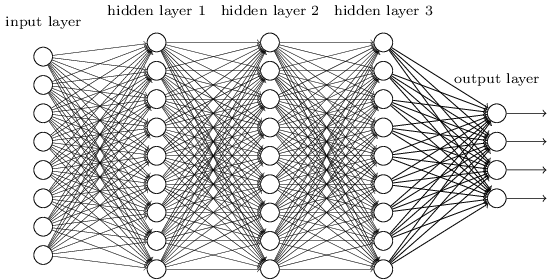
\includegraphics[height=6cm]{img/tikz40.png}
\end{center}

\end{frame}

%%%%%%%%%%%%%%%%%%%%%%%%%%%%%%%%%%%%%%%%%%%%%%%%%%%
\begin{frame}[fragile] \frametitle{} \oldB \small

For an input vector $x$ and a response $y$, we can view a neural network
as simply being something like:
\begin{align}
z^1 &= W^1 a^0 + b^1 \\
a^1 &= \sigma(z^1) \\
z^2 &= W^2 a^1 + b^2 \\
a^2 &= \sigma(z^2) \\
z^3 &= W^3 a^2 + b^3 \\
a^3 &= \sigma(z^3) \\
\text{Cost} &= (y - a^3)^2
\end{align}
Where each level can be described by a \textit{module}. The $z$ layers
are called linear layers, the $a$'s as sigmoid layers, and the last
line is simply the cost function. Notice that the activation functions
are now their own layers, which actually simplifies things mathematically.

\end{frame}

%%%%%%%%%%%%%%%%%%%%%%%%%%%%%%%%%%%%%%%%%%%%%%%%%%%
\begin{frame}[fragile] \frametitle{} \oldB \small

In our formulation, you can see that many of the layers consist of applying
matrix products. When using minibatches, or doing convolution, which we will
see shortly, we will often need to use tensor products. These types of mathematical
operations have highly optimized libraries, often written to take special
advantage of the particular architecture of a given CPU.

As you have already seen on problem set 5, training neural networks can be
quite time consuming. Taking advantage of these benefits is quite important
for even relatively modest training tasks.

\end{frame}

%%%%%%%%%%%%%%%%%%%%%%%%%%%%%%%%%%%%%%%%%%%%%%%%%%%
\begin{frame}[fragile] \frametitle{} \oldB \small

\textbf{\yblue{BLAS: Basic Linear Algebra Subprograms}}

A specification giving consistent API for common operations between
scalars, vectors, and matrices. For example, multiplying a matrix
by a vector. Code written over the BLAS specification can be recompiled
with a specific version of BLAS optimized for a given system. For example,
R and NumPy can both be compiled with custom BLAS implementations.

\end{frame}

%%%%%%%%%%%%%%%%%%%%%%%%%%%%%%%%%%%%%%%%%%%%%%%%%%%
\begin{frame}[fragile] \frametitle{} \oldB \small

\textbf{\yblue{BLAS Implementations}}

Popular implementations include:
\begin{itemize}
\item Netlib BLAS
\item OpenBLAS
\item Automatically Tuned Linear Algebra Software (ATLAS)
\item Intel's Math Kernel Library (MKL)
\end{itemize}

\end{frame}

%%%%%%%%%%%%%%%%%%%%%%%%%%%%%%%%%%%%%%%%%%%%%%%%%%%
\begin{frame}[fragile] \frametitle{} \oldB \small

\textbf{\yblue{General Purpose GPU Programming}}

For years, specialized chips have been developed specifically for
doing fast matrix operations. This research was driven by the need
to offload compute heavy graphics functions from the main CPU onto
a specialized GPU. These have recently been marketed for general
purpose programming, with chips (termed GPGPUs) now being specifically
built and designed for such tasks.

\begin{center}
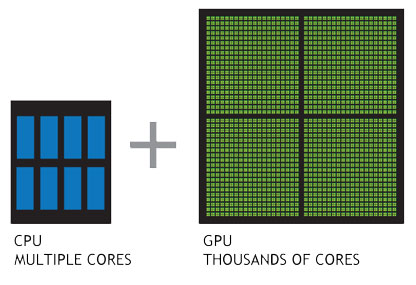
\includegraphics[height=4.5cm]{img/gpgpu.jpg}
\end{center}

\end{frame}

%%%%%%%%%%%%%%%%%%%%%%%%%%%%%%%%%%%%%%%%%%%%%%%%%%%
\begin{frame}[fragile] \frametitle{} \oldB \small

\textbf{\yblue{Example: NVIDIA Tesla}}

These are now virtually required for doing cutting-edge neural network
research:

\begin{center}
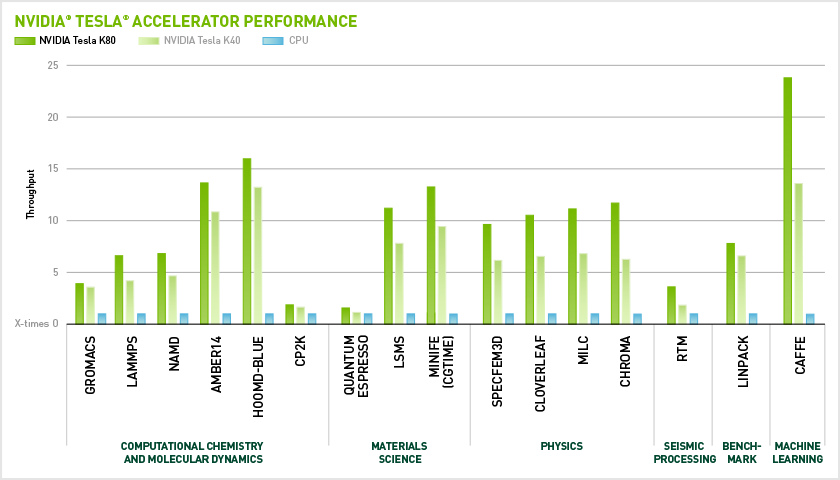
\includegraphics[height=6cm]{img/tesla.png}
\end{center}

\end{frame}

%%%%%%%%%%%%%%%%%%%%%%%%%%%%%%%%%%%%%%%%%%%%%%%%%%%
\begin{frame}[fragile] \frametitle{} \oldB \small

\textbf{\yblue{BLAS and GPGPUs}}

Libraries such as CULA, cuBLAS, cuSPARSE, and LibSciACC provide BLAS
and other functionalities using GPU chips.

\end{frame}

%%%%%%%%%%%%%%%%%%%%%%%%%%%%%%%%%%%%%%%%%%%%%%%%%%%
\begin{frame}[fragile] \frametitle{} \oldB \small

\textbf{\yblue{Neural network software / libraries}}

Back to neural networks, many libraries have been written for training
classes of neural networks. Most of these try to support custom BLAS
implementations, with the possibility of being compiled to a GPU. As
understanding the landscape is important, I'll explain some of the
currently popular examples and give my personal thoughts on them.

\end{frame}

%%%%%%%%%%%%%%%%%%%%%%%%%%%%%%%%%%%%%%%%%%%%%%%%%%%
\begin{frame}[fragile] \frametitle{} \oldB \small


\includegraphics[width=\textwidth]{img/torch.pdf}

\end{frame}

%%%%%%%%%%%%%%%%%%%%%%%%%%%%%%%%%%%%%%%%%%%%%%%%%%%
\begin{frame}[fragile] \frametitle{} \oldB \small

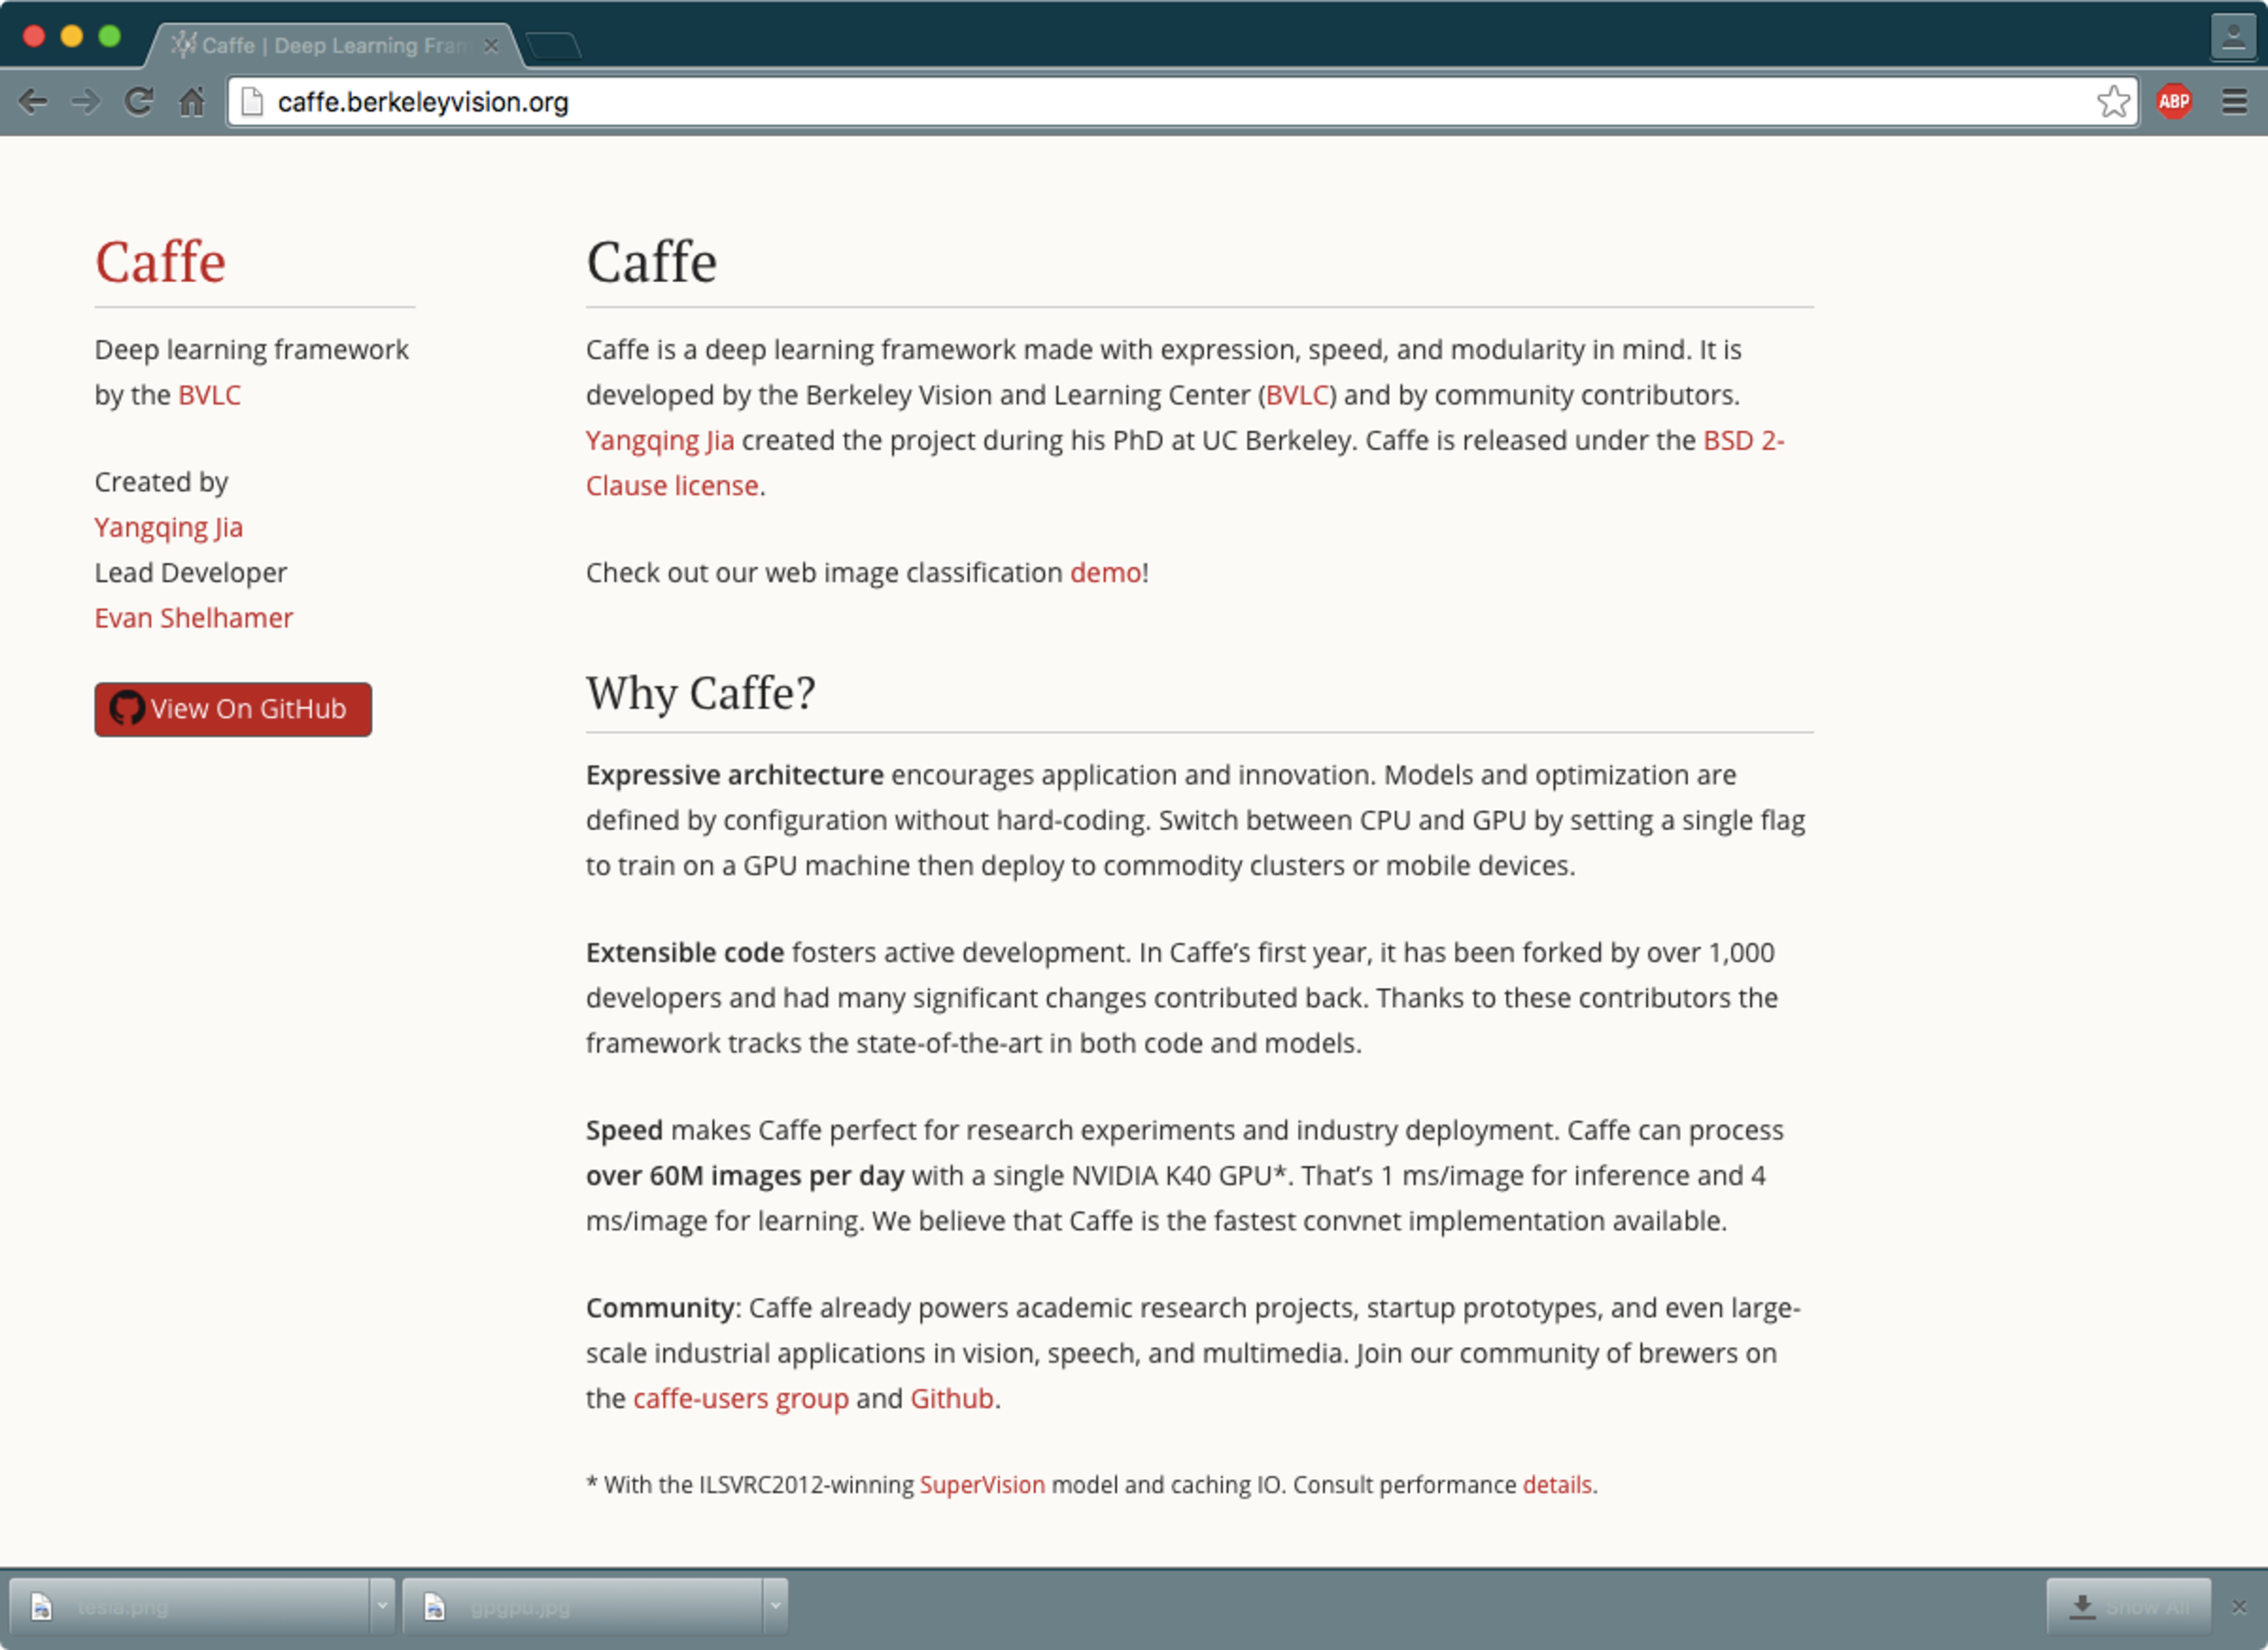
\includegraphics[width=\textwidth]{img/caffee.pdf}

\end{frame}

%%%%%%%%%%%%%%%%%%%%%%%%%%%%%%%%%%%%%%%%%%%%%%%%%%%
\begin{frame}[fragile] \frametitle{} \oldB \small

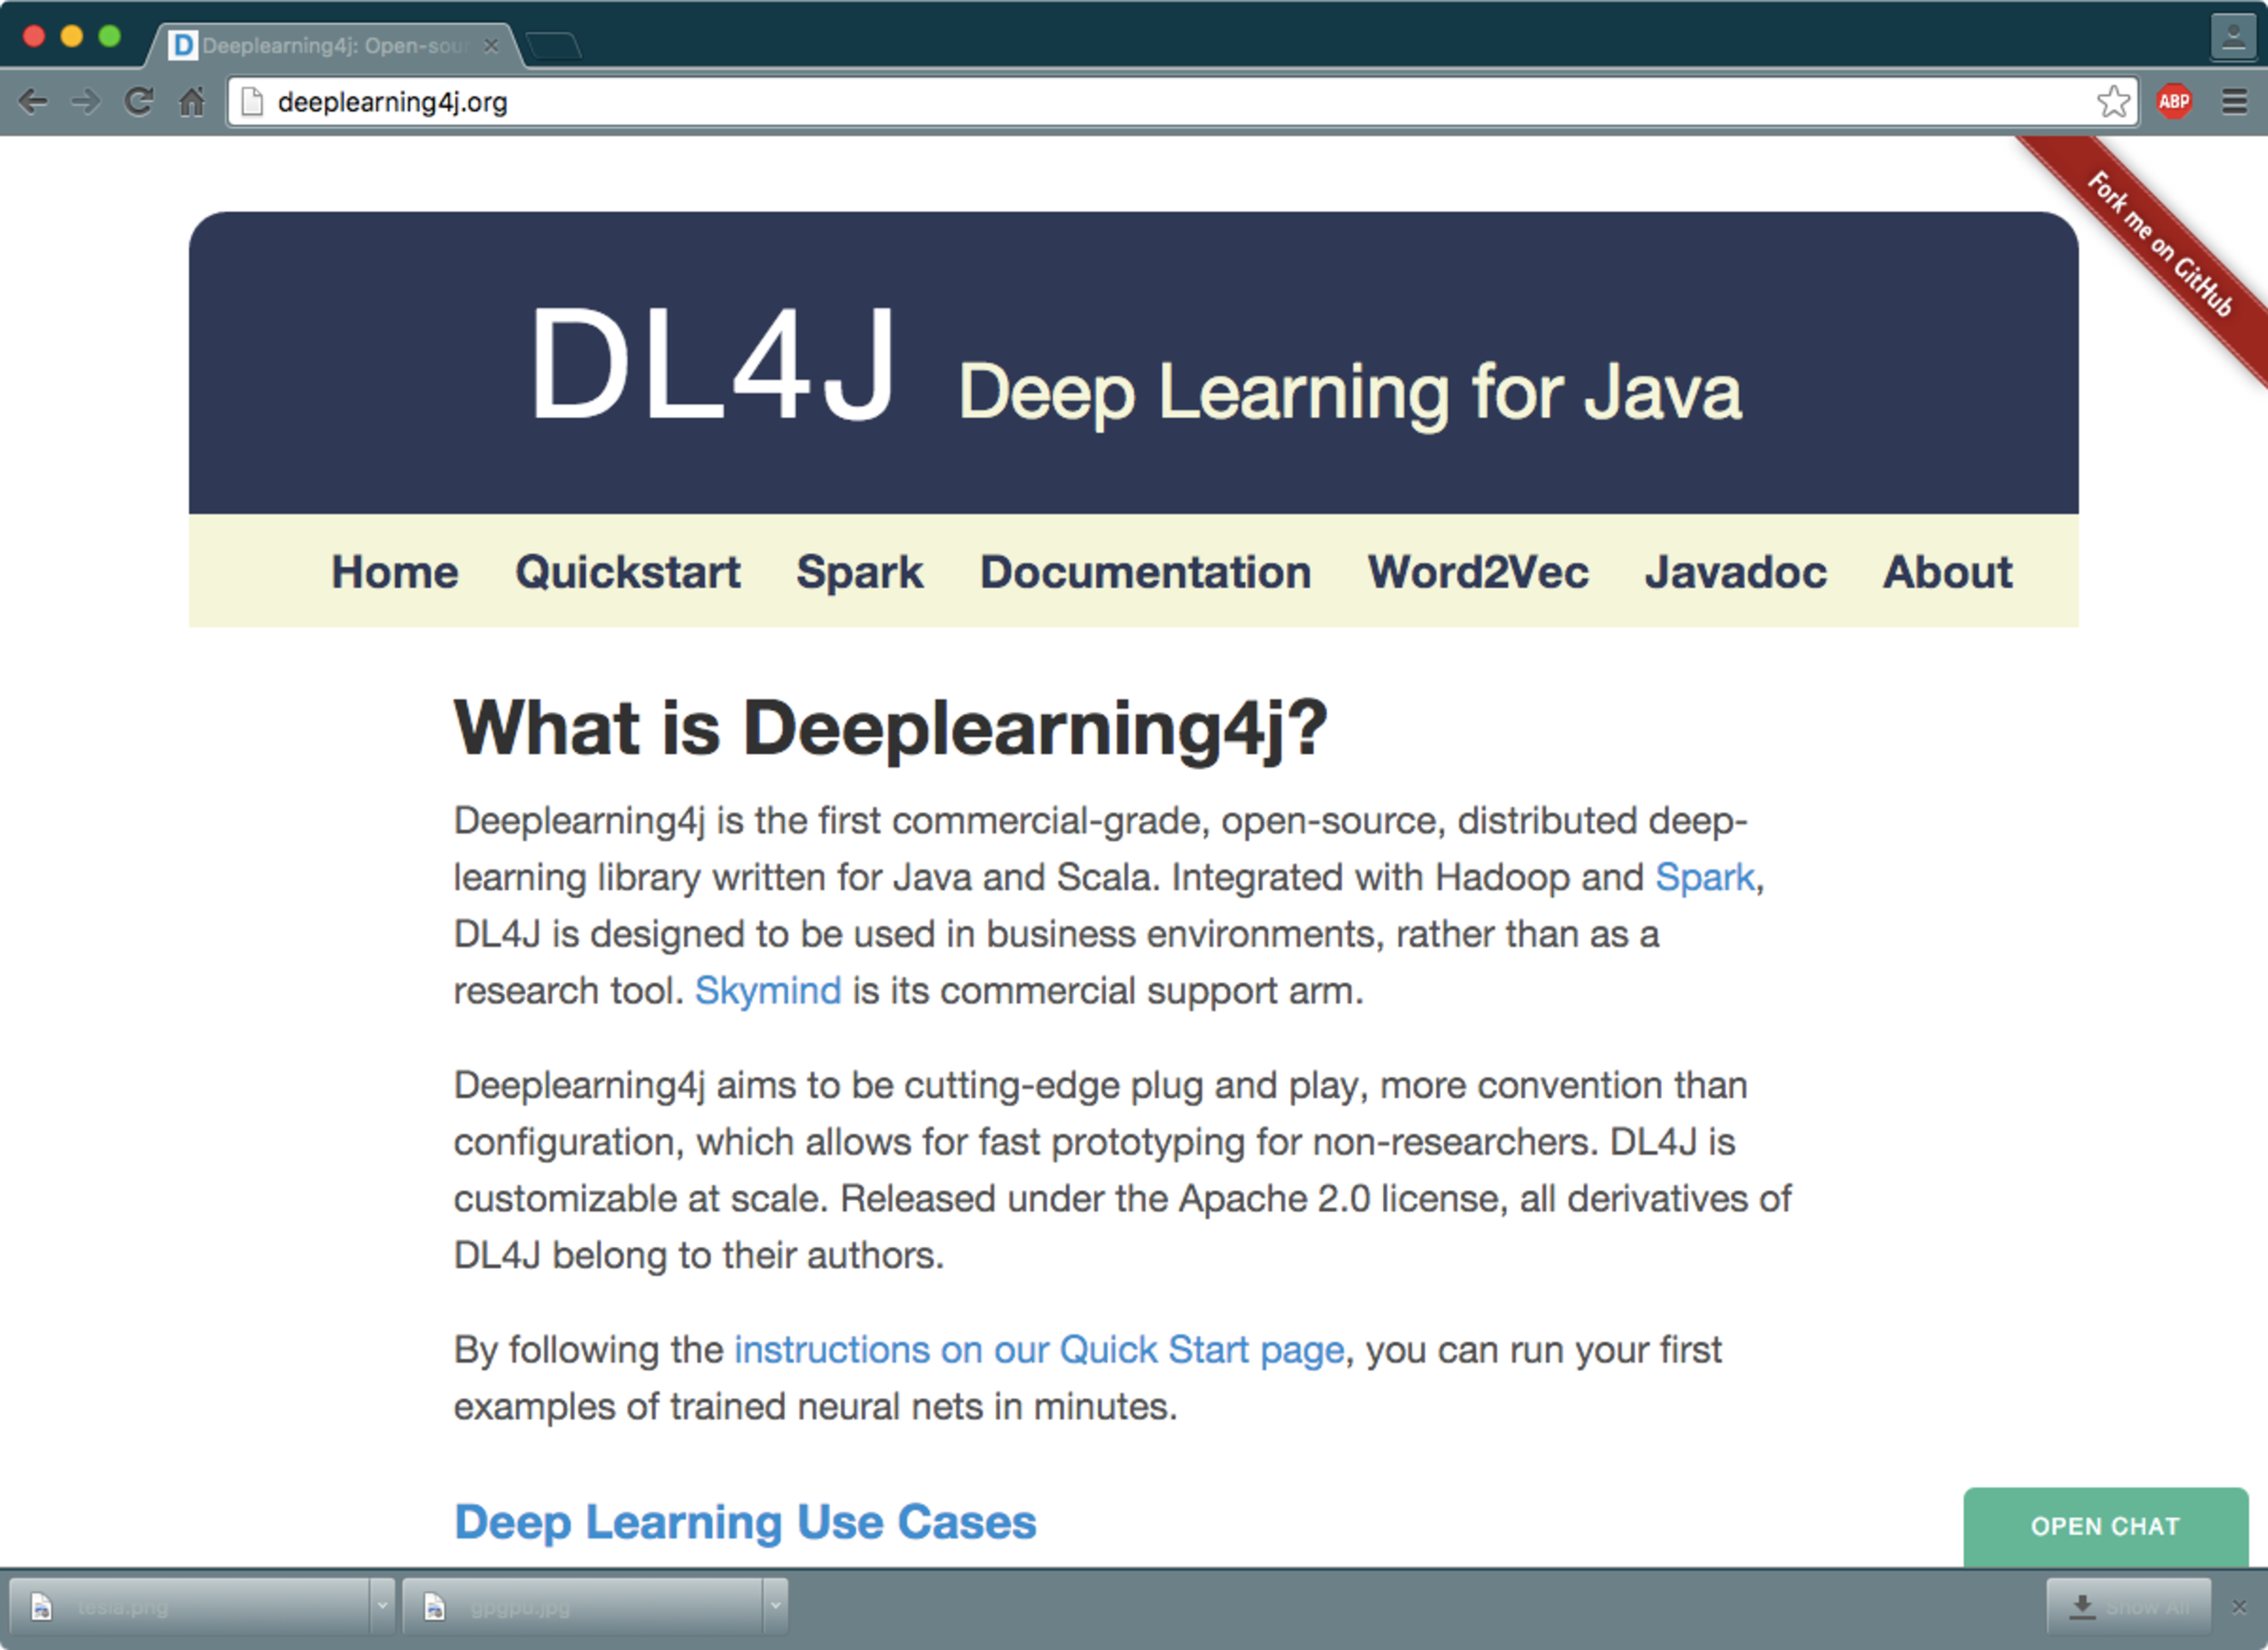
\includegraphics[width=\textwidth]{img/deeplearning.pdf}

\end{frame}

%%%%%%%%%%%%%%%%%%%%%%%%%%%%%%%%%%%%%%%%%%%%%%%%%%%
\begin{frame}[fragile] \frametitle{} \oldB \small

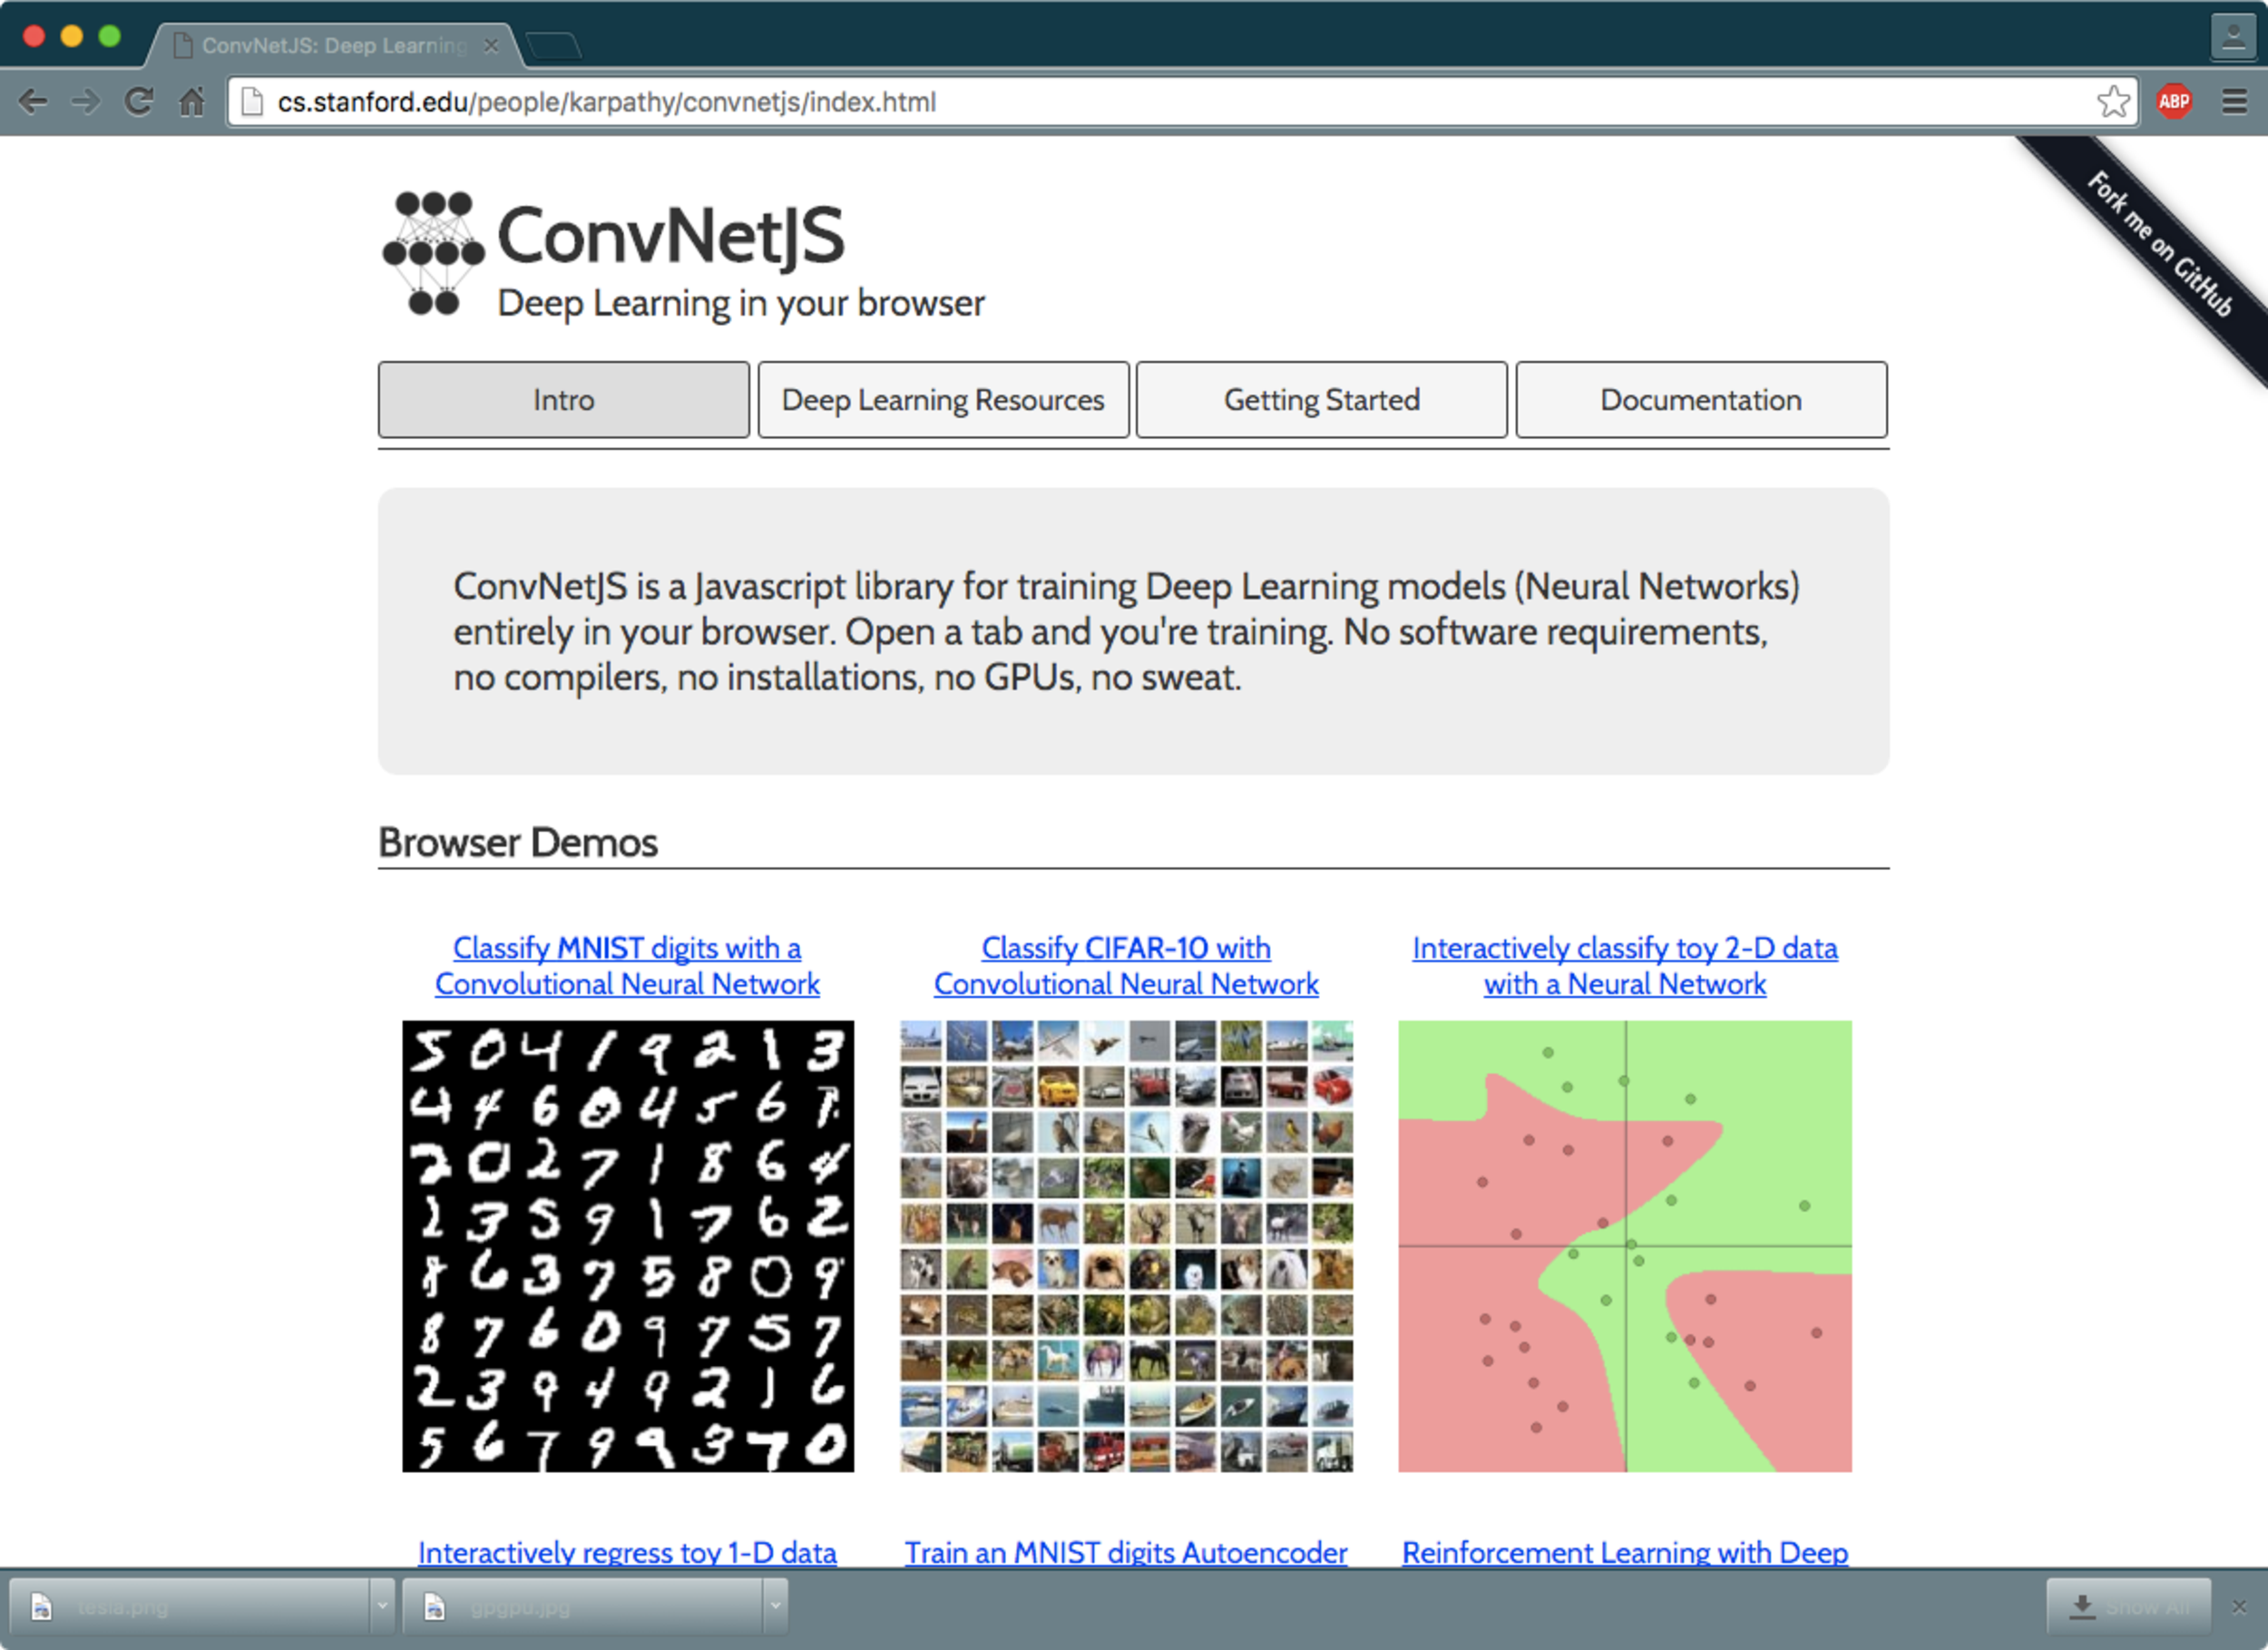
\includegraphics[width=\textwidth]{img/convnetjs.pdf}

\end{frame}

%%%%%%%%%%%%%%%%%%%%%%%%%%%%%%%%%%%%%%%%%%%%%%%%%%%
\begin{frame}[fragile] \frametitle{} \oldB \small

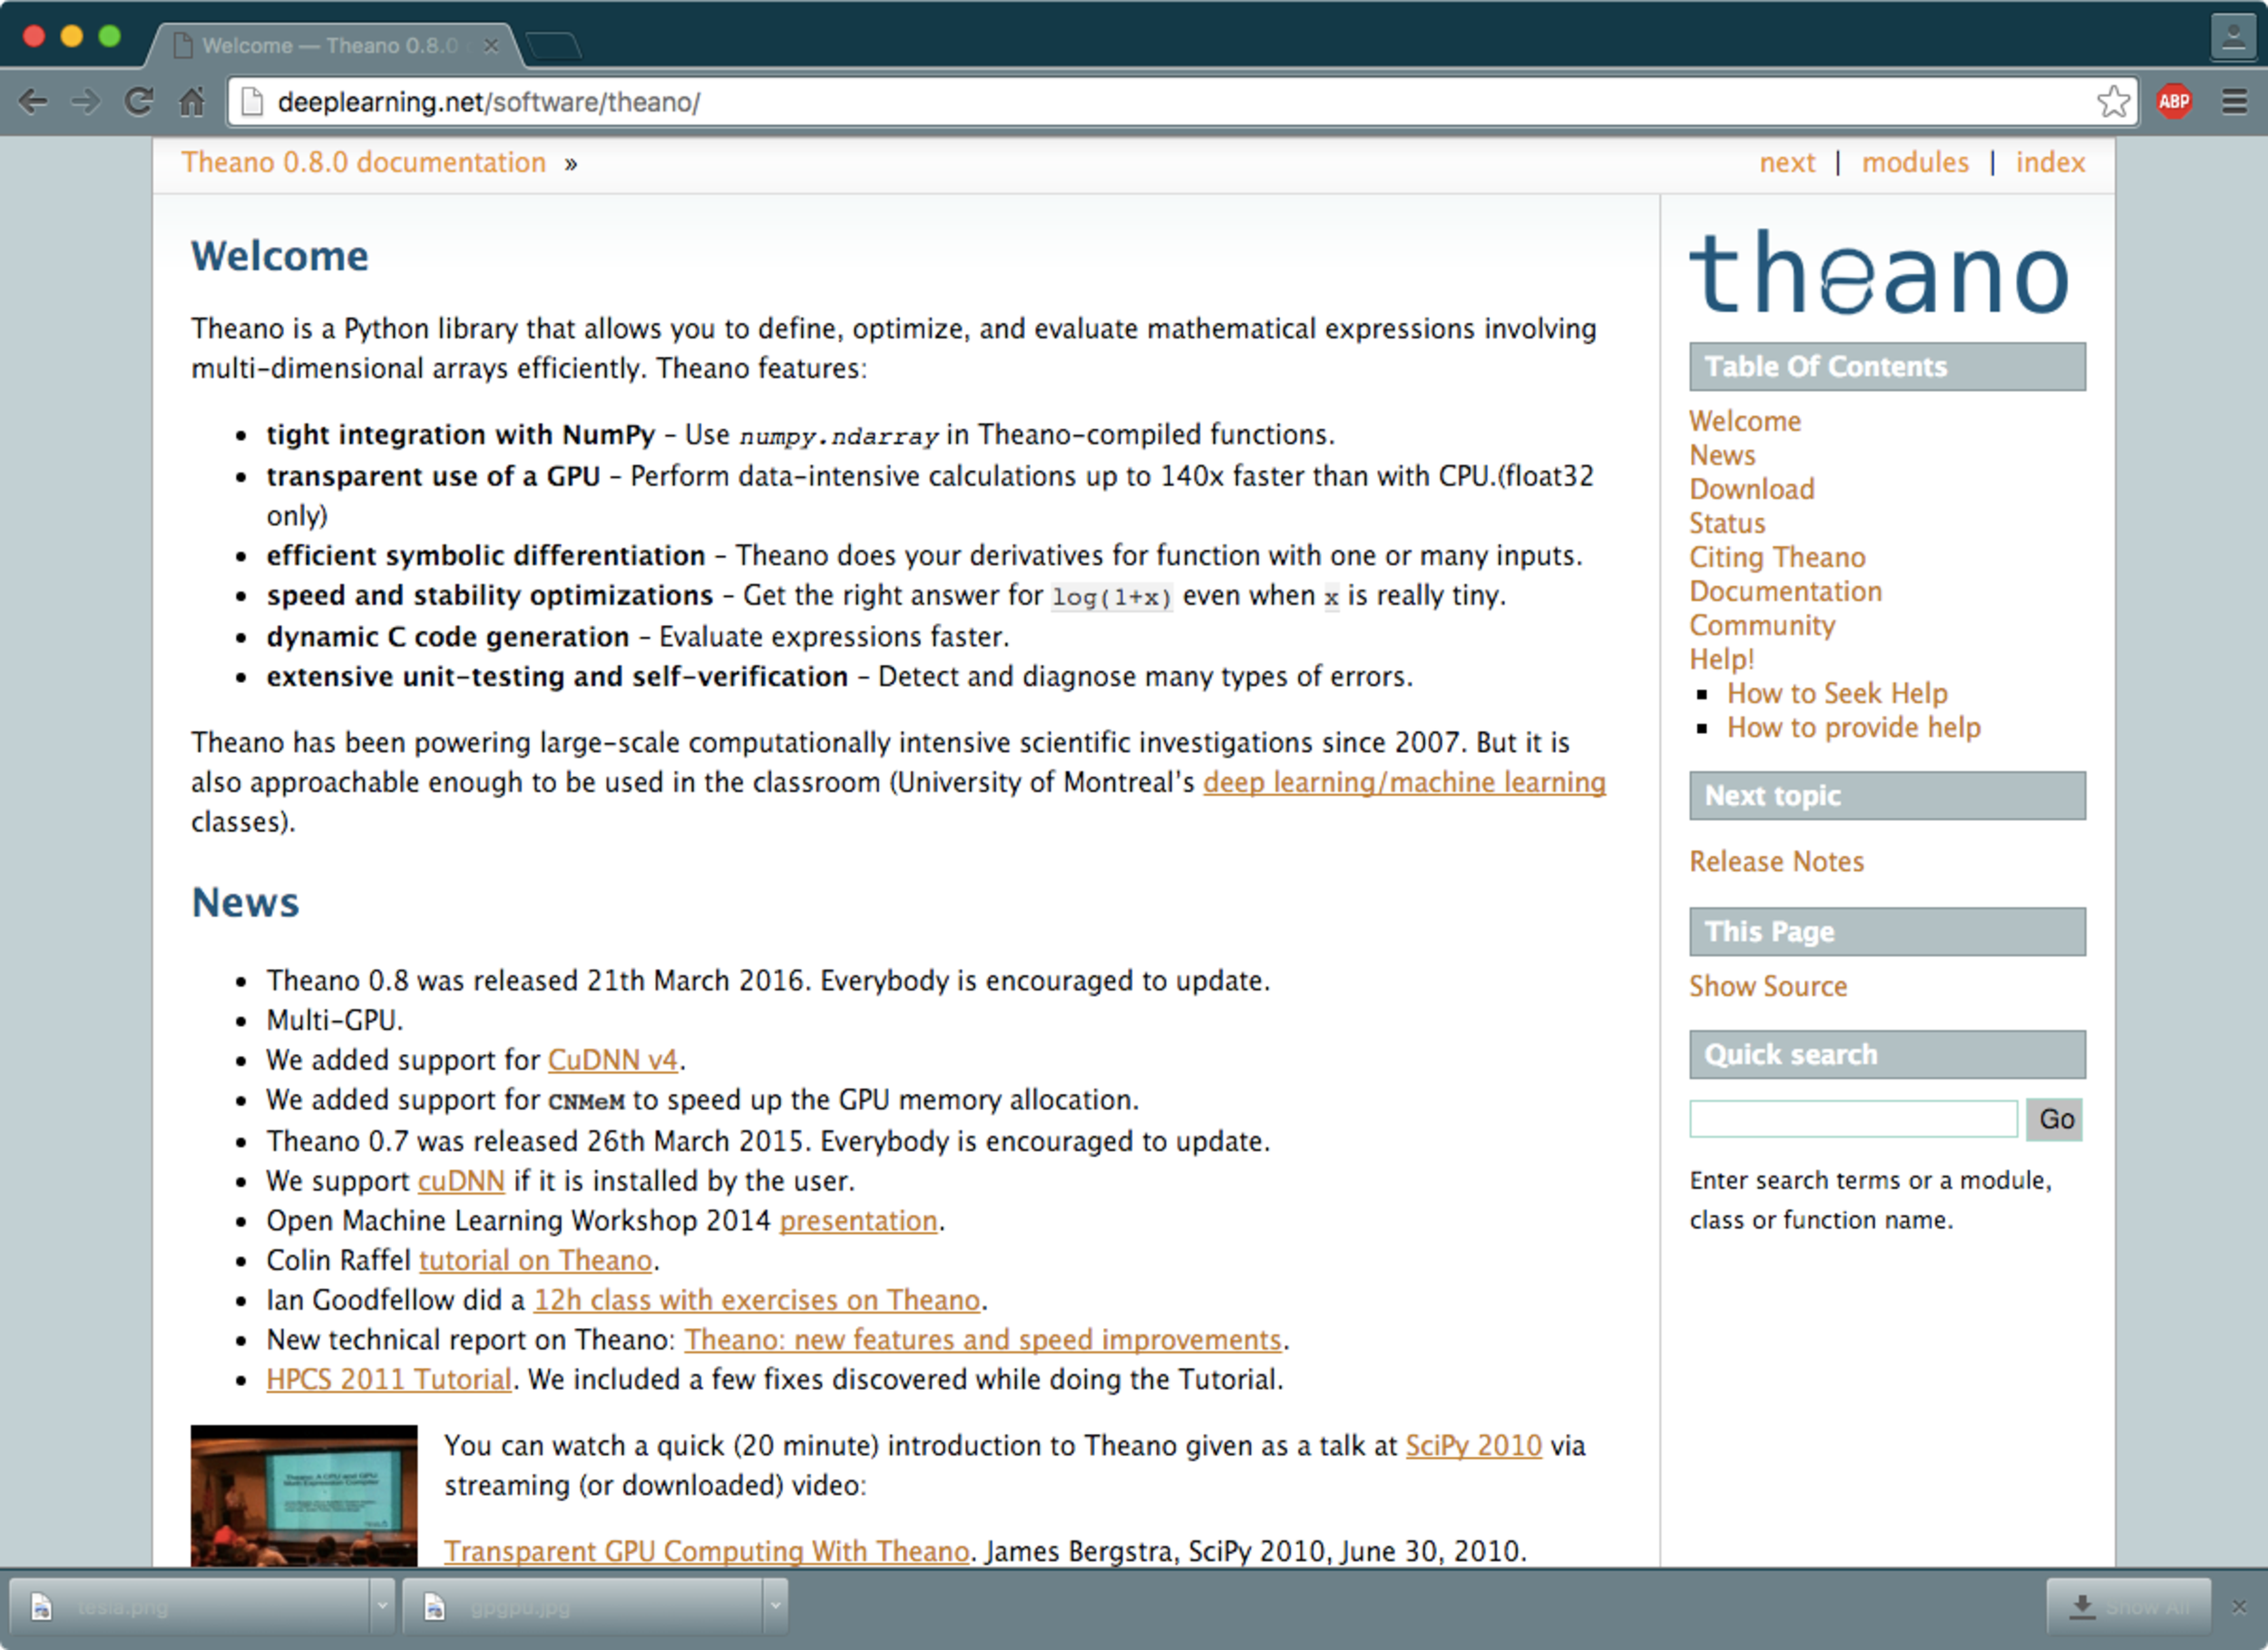
\includegraphics[width=\textwidth]{img/theano.pdf}

\end{frame}

%%%%%%%%%%%%%%%%%%%%%%%%%%%%%%%%%%%%%%%%%%%%%%%%%%%
\begin{frame}[fragile] \frametitle{} \oldB \small

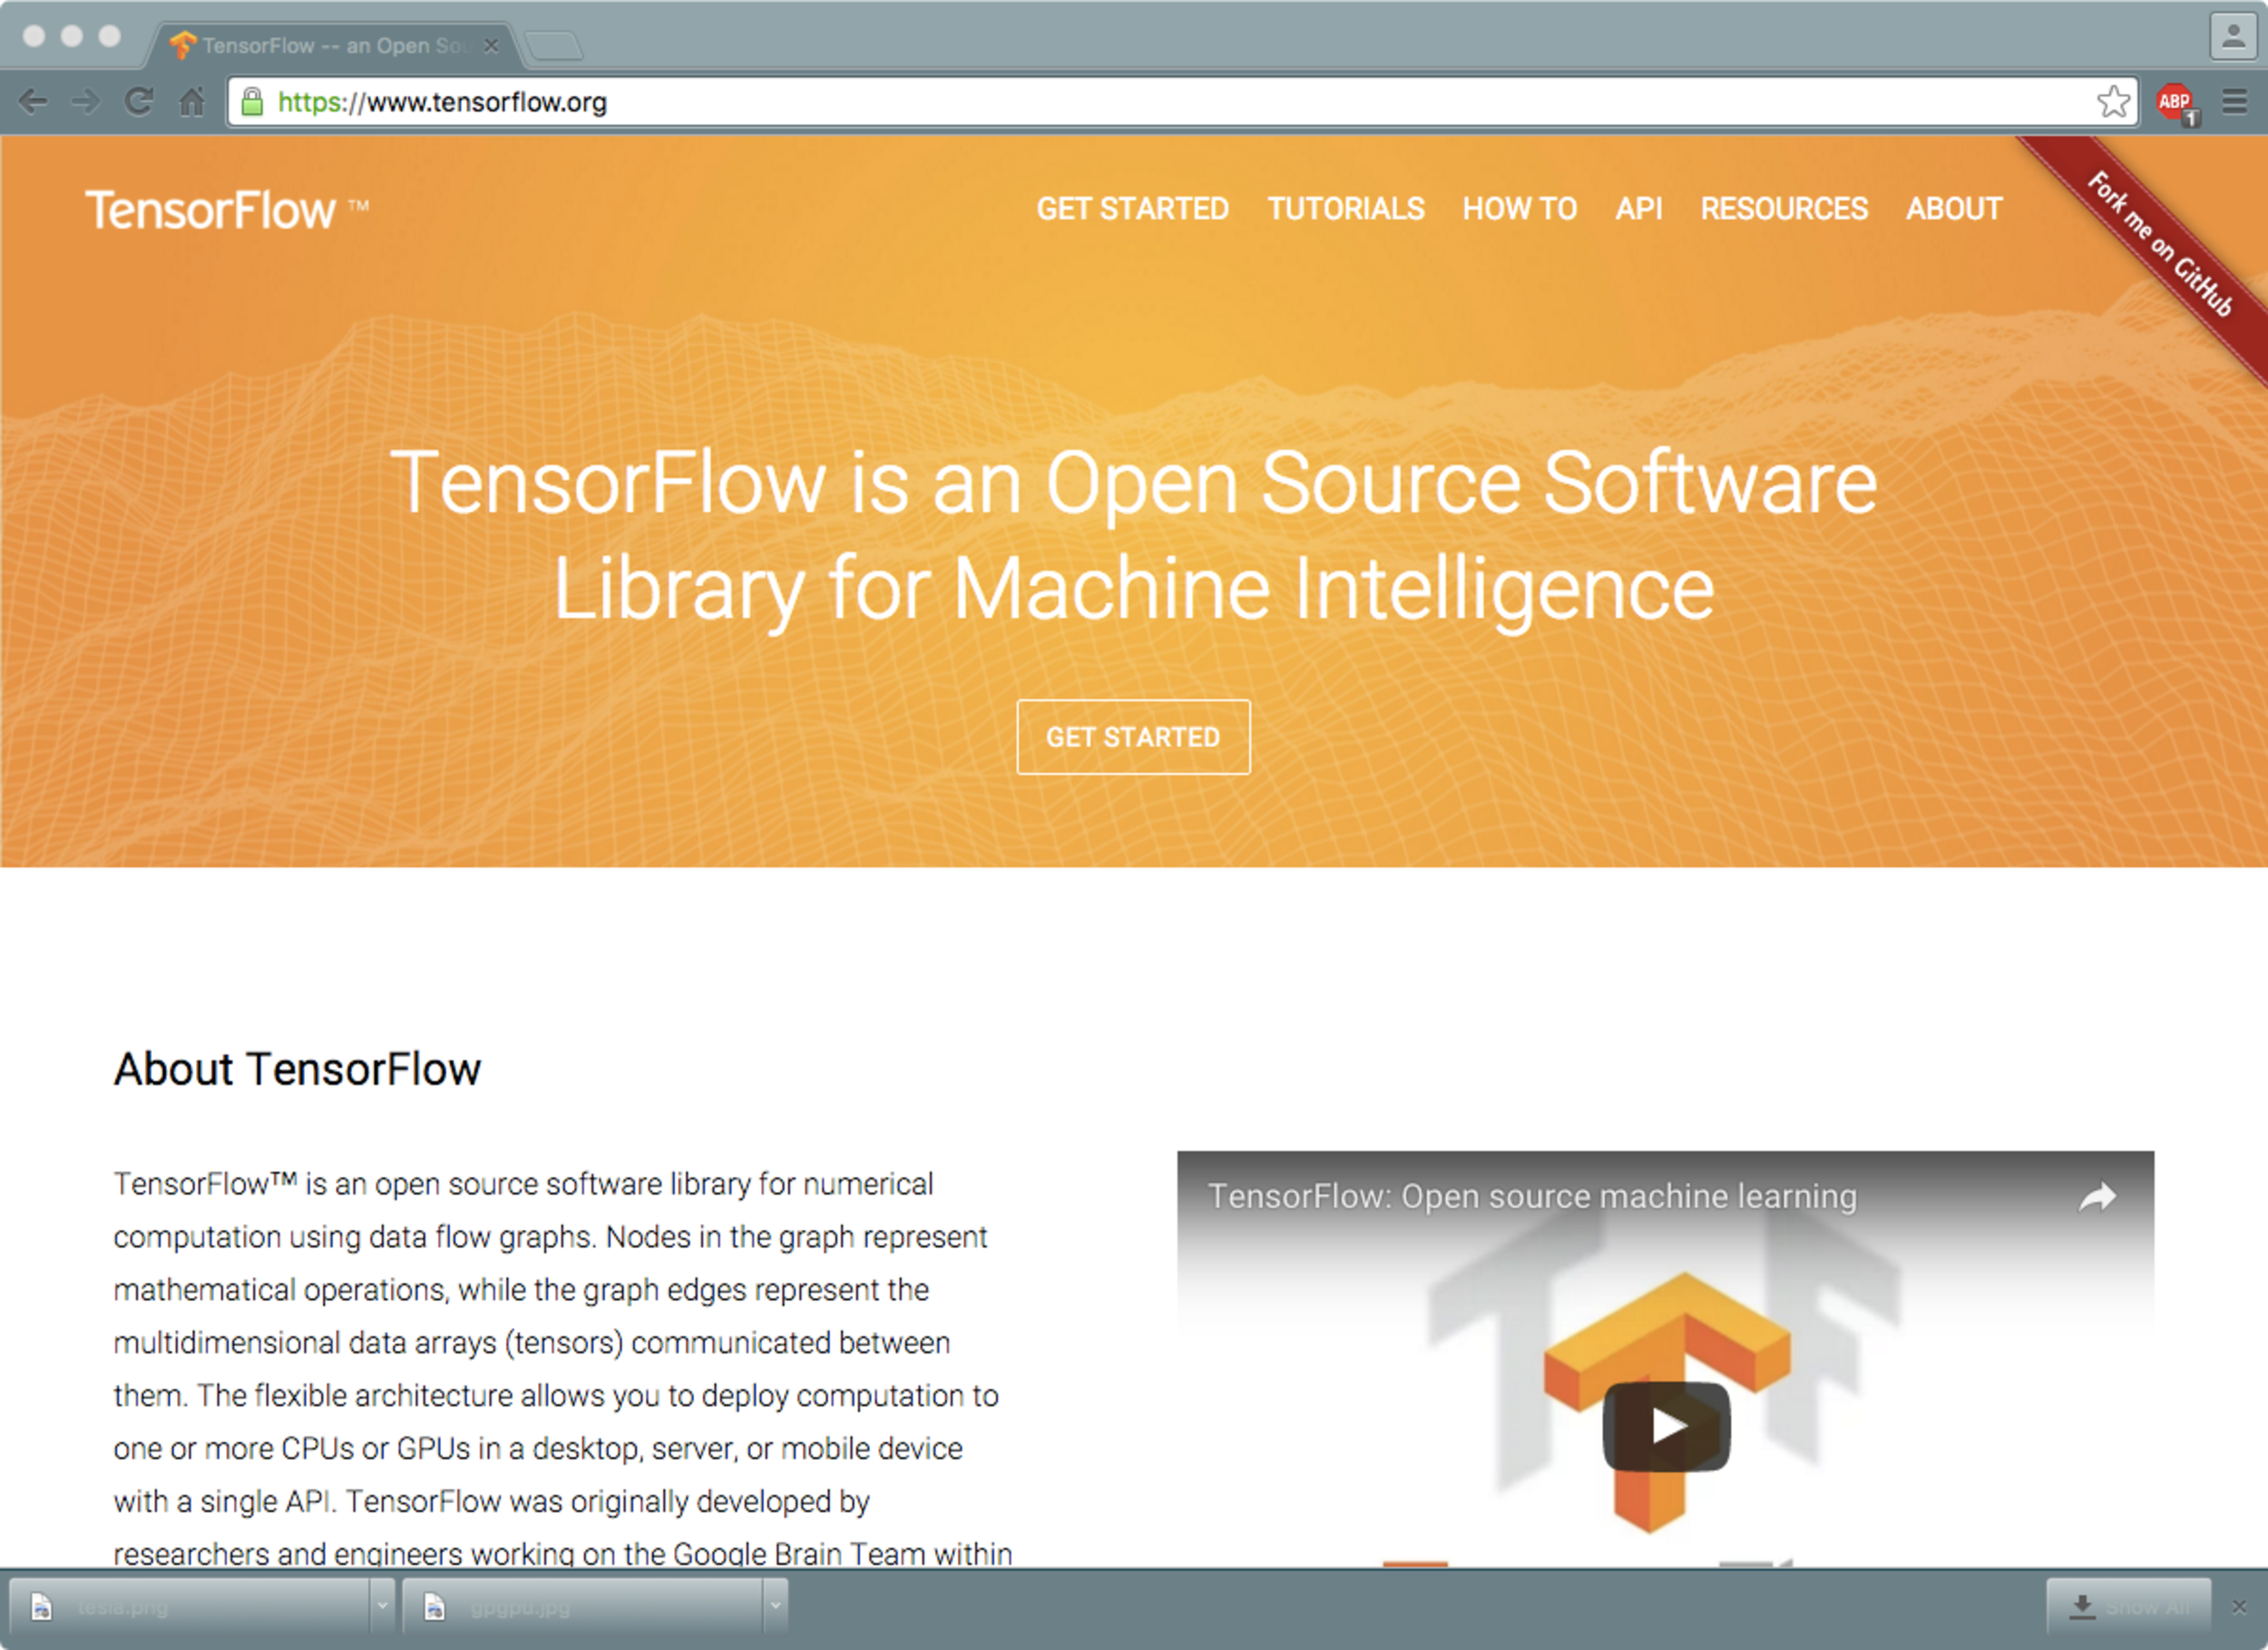
\includegraphics[width=\textwidth]{img/tensorflow.pdf}

\end{frame}

%%%%%%%%%%%%%%%%%%%%%%%%%%%%%%%%%%%%%%%%%%%%%%%%%%%
\begin{frame}[fragile] \frametitle{} \oldB \small

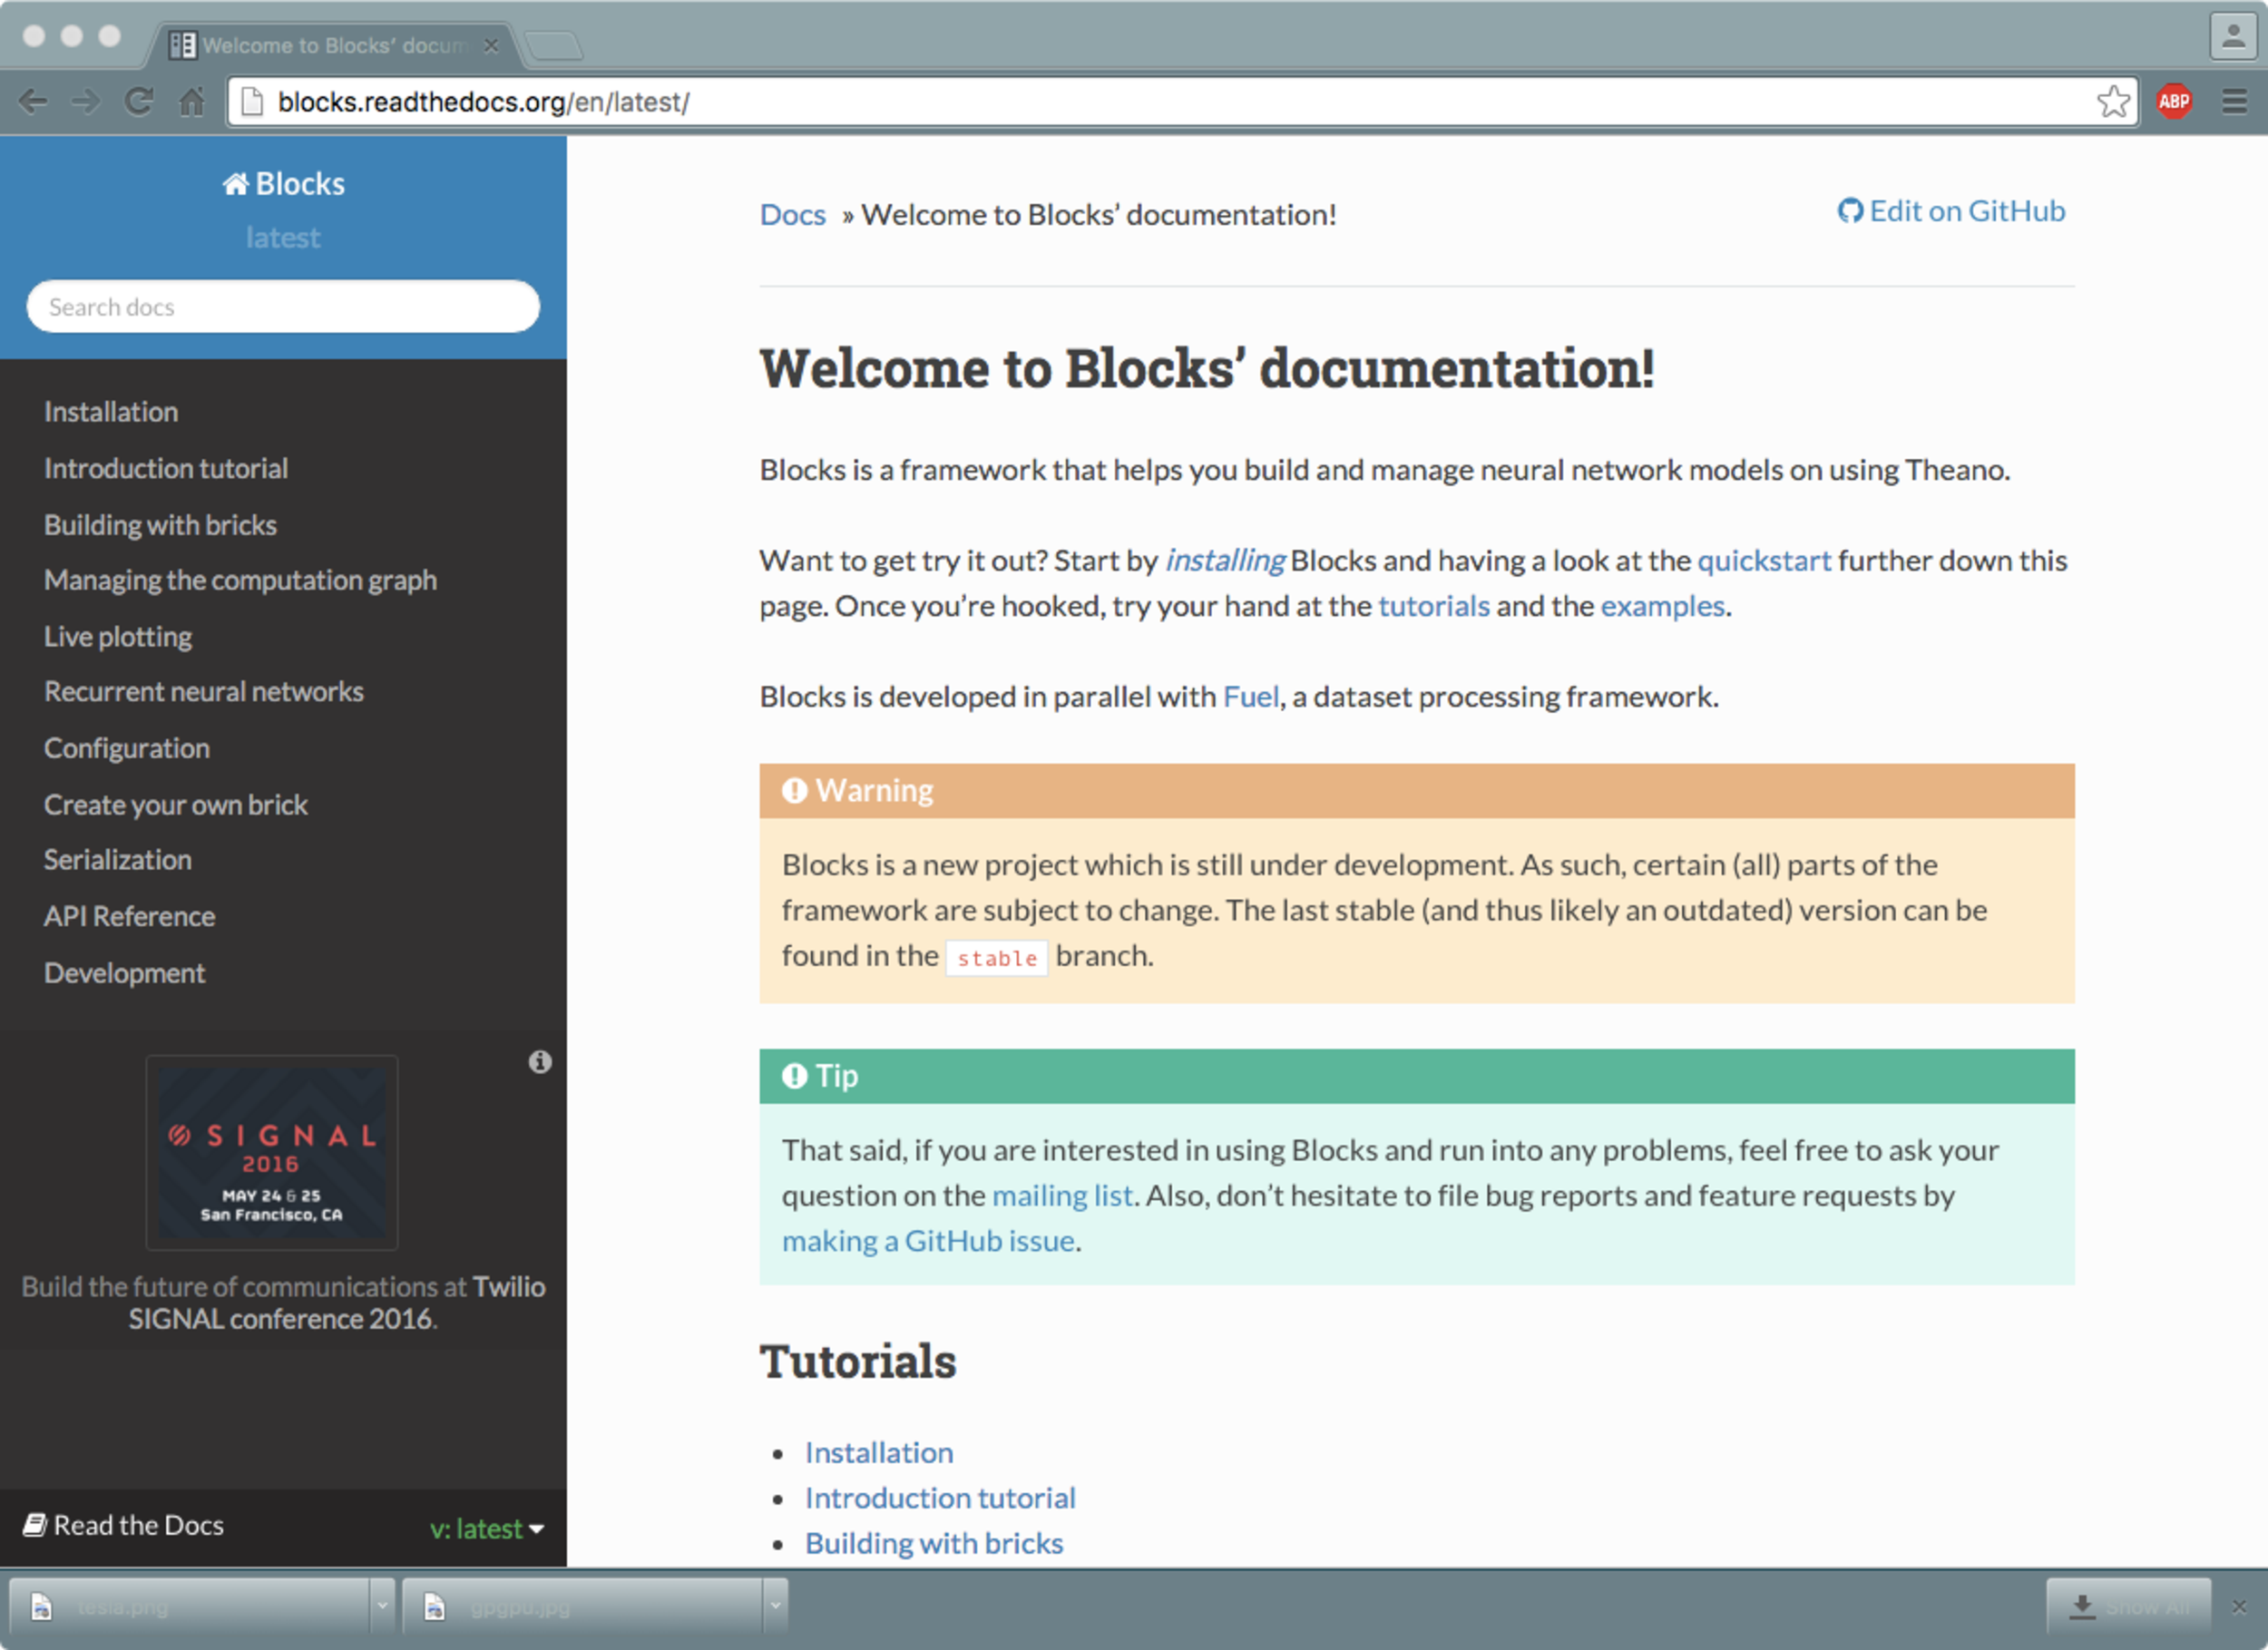
\includegraphics[width=\textwidth]{img/blocks.pdf}

\end{frame}

%%%%%%%%%%%%%%%%%%%%%%%%%%%%%%%%%%%%%%%%%%%%%%%%%%%
\begin{frame}[fragile] \frametitle{} \oldB \small

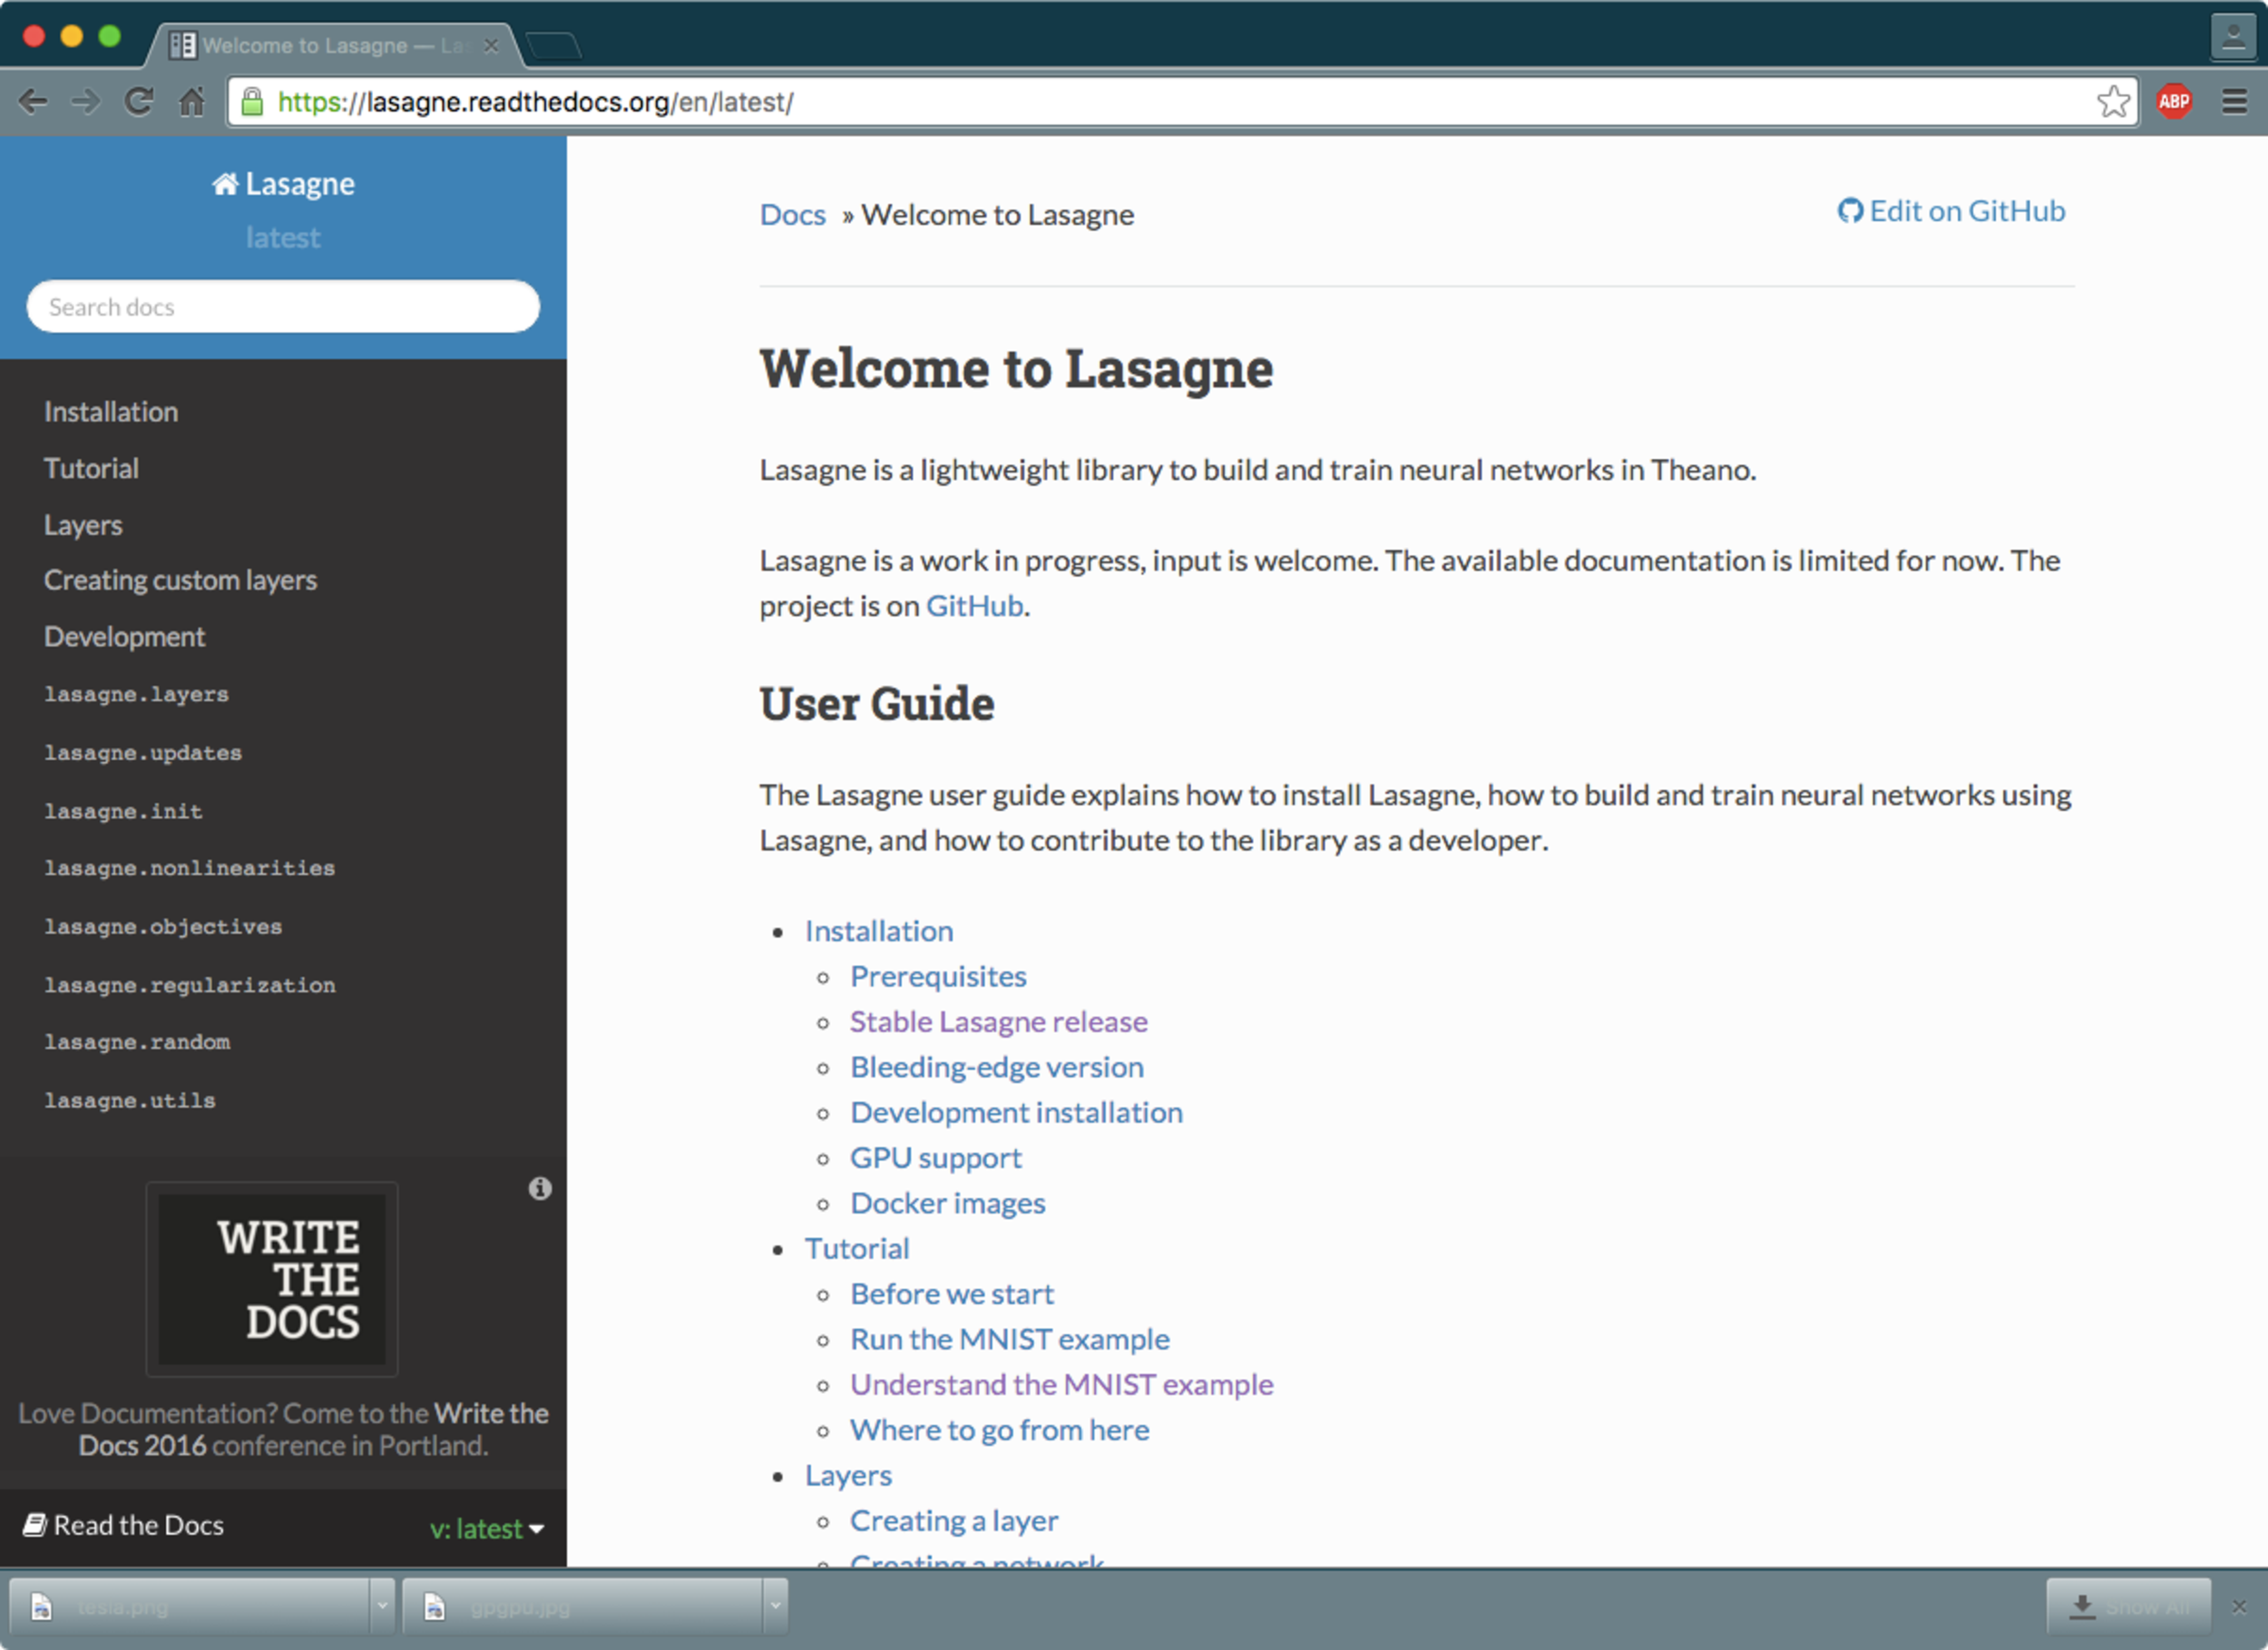
\includegraphics[width=\textwidth]{img/lasagna.pdf}

\end{frame}

%%%%%%%%%%%%%%%%%%%%%%%%%%%%%%%%%%%%%%%%%%%%%%%%%%%
\begin{frame}[fragile] \frametitle{} \oldB \small

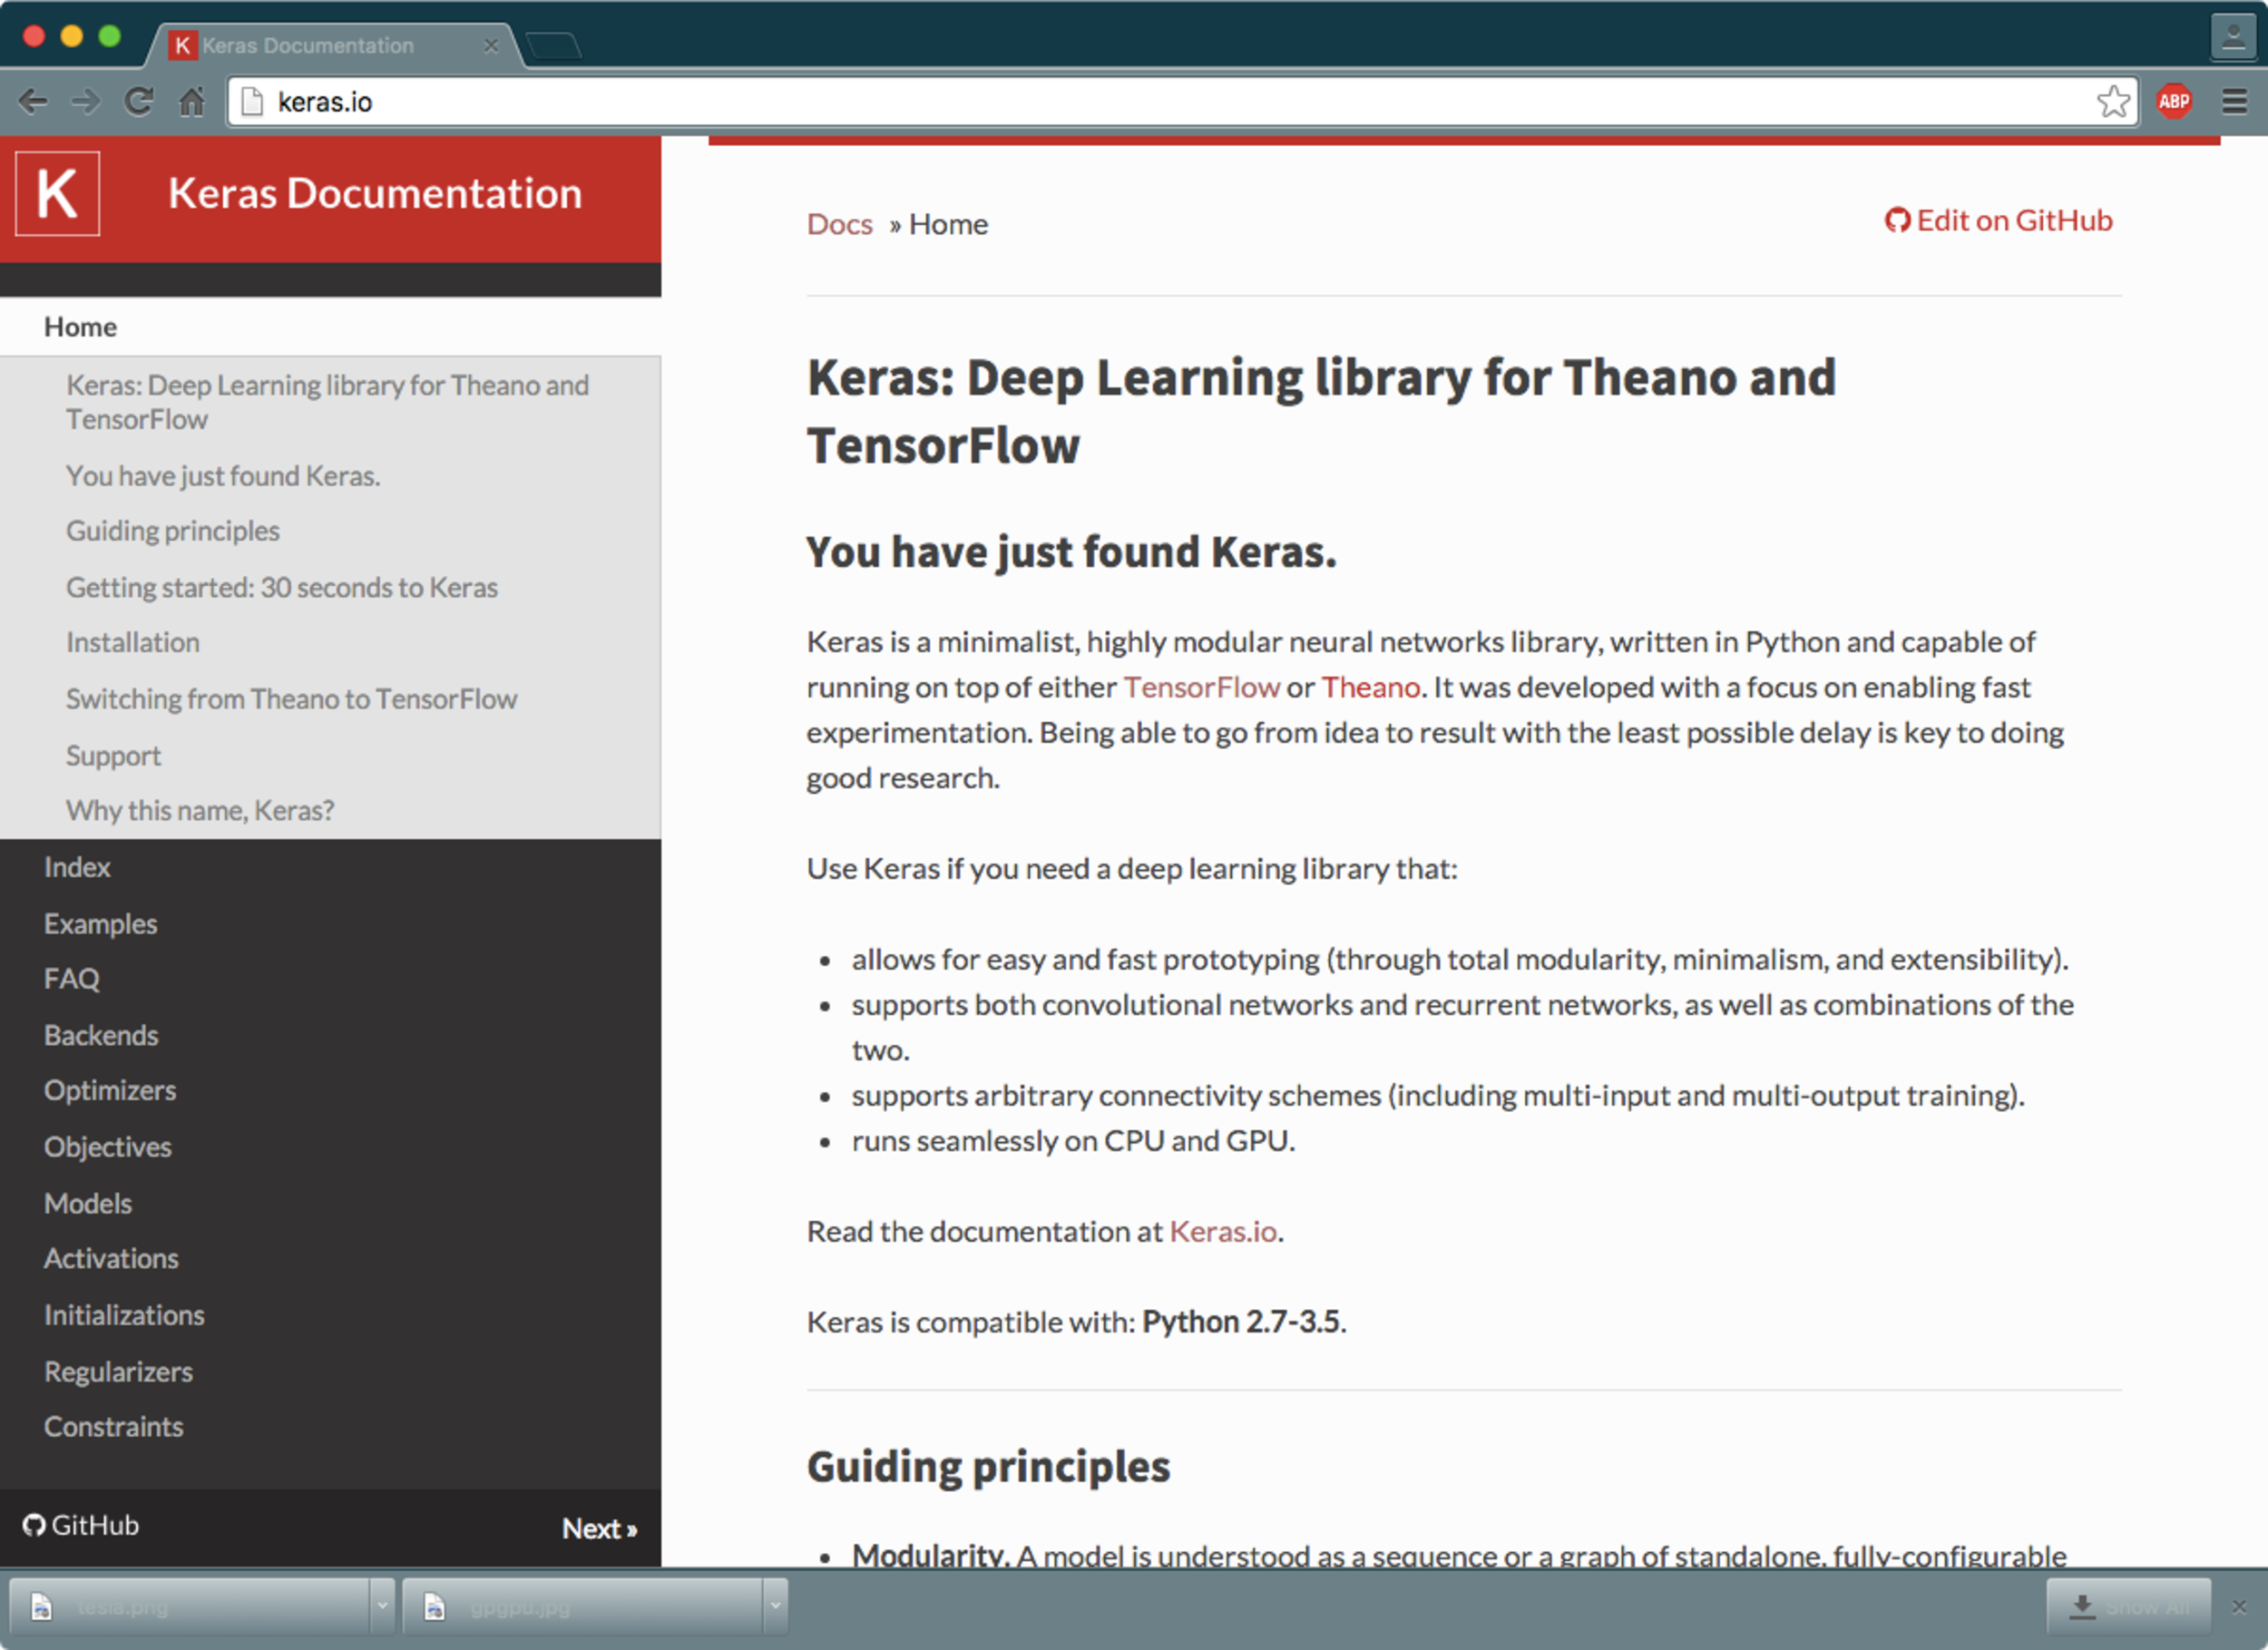
\includegraphics[width=\textwidth]{img/keras.pdf}

\end{frame}

%%%%%%%%%%%%%%%%%%%%%%%%%%%%%%%%%%%%%%%%%%%%%%%%%%%
\begin{frame}[fragile] \frametitle{} \oldB \small

\textbf{\yblue{keras}}

We are going to use the keras library in this course;
it uses python (a language many of you are familiar with
and is relatively close to R), is easy to install across
different operating systems, and supports both convolution
and recurrent neural networks. As it uses either the Theano
or TensorFlow backends, it is likely to be relatively up-to-date for at
least the immediate future.

\end{frame}

%%%%%%%%%%%%%%%%%%%%%%%%%%%%%%%%%%%%%%%%%%%%%%%%%%%
\begin{frame}[fragile] \frametitle{} \oldB \small

\textbf{\yblue{Importing functions}}

I will let you all consult the keras website for getting
the library installed on your machine. Before diving into
the tutorial, I wanted to make a note of a difference
between python and R.

In R, when we call \texttt{library} or \texttt{require}
with a package name, all of the public functions in that
package are added directly to the search path. For example:
\begin{verbatim}
> library(class)
> knn(train, test, cl, k = 3, prob=TRUE)
\end{verbatim}

\end{frame}

%%%%%%%%%%%%%%%%%%%%%%%%%%%%%%%%%%%%%%%%%%%%%%%%%%%
\begin{frame}[fragile] \frametitle{} \oldB \small

We could instead explicatively call the knn function,
without ever loading the class library, by doing the
following:
\begin{verbatim}
> class::knn(train, test, cl, k = 3, prob=TRUE)
\end{verbatim}
This would work (to the user) exactly the same as the
other form.

\end{frame}

%%%%%%%%%%%%%%%%%%%%%%%%%%%%%%%%%%%%%%%%%%%%%%%%%%%
\begin{frame}[fragile] \frametitle{} \oldB \small

In python, this process works differently. We cannot
call a function without first importing the module
it is contained in. Even once a function is imported,
we still need to explicitly let python know from
which module the function is coming from:
\begin{verbatim}
>>> import numpy
>>> numpy.array((1,2))
array([1, 2])
\end{verbatim}
\pause You can imagine that this can become quite verbose,
and it is possible the give a shortened name to the module
instead:
\begin{verbatim}
>>> import numpy as np
>>> np.array((1,2))
array([1, 2])
\end{verbatim}
With some abbreviations, such as this one, becoming fairly
canonical.

\end{frame}

%%%%%%%%%%%%%%%%%%%%%%%%%%%%%%%%%%%%%%%%%%%%%%%%%%%
\begin{frame}[fragile] \frametitle{} \oldB \small

It is possible to avoid having to type even this shortened
form, by explicitly importing a given function:
\begin{verbatim}
>>> from numpy import array
>>> array((1,2))
array([1, 2])
\end{verbatim}
\pause Multiple functions can be imported all at once:
\begin{verbatim}
>>> from numpy import array, zeros
>>> zeros((3,4))
array([[ 0.,  0.,  0.,  0.],
       [ 0.,  0.,  0.,  0.],
       [ 0.,  0.,  0.,  0.]])
\end{verbatim}

\end{frame}

%%%%%%%%%%%%%%%%%%%%%%%%%%%%%%%%%%%%%%%%%%%%%%%%%%%
\begin{frame}[fragile] \frametitle{} \oldB \small

It is possible, but considered very poor form, to
load all of the functions from a module by doing:
\begin{verbatim}
>>> from numpy import *
>>> array((1,2))
array([1, 2])
\end{verbatim}
Which gives a more R-like behavior.

\end{frame}

%%%%%%%%%%%%%%%%%%%%%%%%%%%%%%%%%%%%%%%%%%%%%%%%%%%
\begin{frame}[fragile] \frametitle{} \oldB \small

Finally, some modules contain additional submodules.
For example, SciPy has a stats submodule:
\begin{verbatim}
>>> from scipy.stats import beta
>>> a, b = 1., 2.
>>> beta.rvs(a, b, size=4)
array([ 0.04541352,  0.82622532,  0.10097377,  0.37001809])
\end{verbatim}
You can generally think of these as completely
independent modules.

\end{frame}

%%%%%%%%%%%%%%%%%%%%%%%%%%%%%%%%%%%%%%%%%%%%%%%%%%%
\begin{frame}[fragile] \frametitle{} \oldB \small

\textbf{\yblue{Minimal working example}}

Speaking of importing functions from python modules,
let's load these four functions from keras:
\begin{verbatim}
>>> from keras.models import Sequential
>>> from keras.layers.core import Dense, Activation
>>> from keras.optimizers import SGD
\end{verbatim}

\end{frame}

%%%%%%%%%%%%%%%%%%%%%%%%%%%%%%%%%%%%%%%%%%%%%%%%%%%
\begin{frame}[fragile] \frametitle{} \oldB \small

\textbf{\yblue{Minimal working example, cont.}}

We start by constructing a Sequential model, and
adding three layers to it: a linear, or dense, layer;
the activation layer; and the output layer.
\begin{verbatim}
>>> model = Sequential()
>>> model.add(Dense(512, input_shape=(28 * 28,)))
>>> model.add(Activation("sigmoid"))
>>> model.add(Dense(10))
\end{verbatim}
The input shape parameter needs to be set for the
first layer, but can be inferred for all of the other
layers.

\end{frame}

%%%%%%%%%%%%%%%%%%%%%%%%%%%%%%%%%%%%%%%%%%%%%%%%%%%
\begin{frame}[fragile] \frametitle{} \oldB \small

\textbf{\yblue{Minimal working example, cont.}}

Now, we will compile the model (this may take a minute
or more) using stochastic gradient descent.
\begin{verbatim}
>>> sgd = SGD(lr = 0.02, momentum = 0.01, nesterov = True)
>>> model.compile(loss='mse', optimizer=sgd)
\end{verbatim}
By setting various environment variables, we could do this
over Tensorflow or Theano, and could make it run over
various CPU or GPU architectures.

\end{frame}

%%%%%%%%%%%%%%%%%%%%%%%%%%%%%%%%%%%%%%%%%%%%%%%%%%%
\begin{frame}[fragile] \frametitle{} \oldB \small

\textbf{\yblue{Minimal working example, cont.}}

To train the actual model, we run the fit method on
the model, giving the desired batch size and number
of epochs:
\begin{verbatim}
>>> model.fit(X_train, Y_train, batch_size=32, nb_epoch=25,
...           verbose=1, show_accuracy=True)
\end{verbatim}
This will produce a running output of the model training
process.

\pause Let's now actually run this is the Python interpreter
and see the various advanced features than can be easily added
to adapt the final model.

\end{frame}



\end{document}











